After the thorough requirement analysis in Section \ref{sec::RequirementAnalysis} based on which a concept for the software was derived in Section \ref{sec::Concept}, 
the following section will focus on the implementation of the system components, starting with architectural components as well as utilities provided by SteamVR.
The virtual OT and the design process will then be shortly described.
Afterwards, available user interactions and the concrete implementation details of surgical procedures and visualization tools will be discussed.
Lastly, the work- and interaction flow of the system will be described.

\section{\label{sec::Architecture}Architecture}
As this thesis aims to offer an open-source framework for VR surgery, the most obvious choice for hardware was used.
A combination of commercially available HMDs and open-source software is used to develop an easily accessible framework.
For this thesis, the HTC Vive \cite{Vive} together with the recent Valve Index Controllers \cite{ValveIndex} were used.
However, any commercially available headset and controllers, which is compatible with SteamVR will work with this system.
OpenVR \cite{OpenVR} (also called SteamVR), the from Steam developed open-source framework for VR development, abstracts the HMD and specifics of controllers for the end user.
By utilizing SteamVR, requirement \ref{req::N9} is practically ensured.

Since running virtual reality software is computationally expensive, a desktop computer with the following hardware is recommended to comply with the given robustness 
and responsiveness requirements (\ref{req::N4}, \ref{req::N6}):

\begin{compactenum}[label=(\alph*)]
    \item Graphics Card: Nvidia GTX 1060 or equivalent
    \item CPU: Intel i5-4590 / AMD Ryzen5 1500X
    \item Memory (RAM): 8GB+
\end{compactenum}

%SteamVR
The VR software was developed using Unity3D (LTS 2018.4), which is broadly accepted by the community and seen as an easy to learn tool, with many tutorials and community 
support for learning \cite{bartneck2015robot}.
\\ Inside of Unity, the OpenVR Toolkit provided by SteamVR is used.
SteamVR consists of an interaction system in which button presses are mapped to actions.
By implementing features with actions instead of button presses in mind, controls are abstracted for any kind of input device.
Mappings can then be customized to user needs, although defaults are available for every controller supported.
\\ Additionally, the interaction system found in SteamVR will be utilized for this thesis, as it provides many functionalities to comply with requirement \ref{req::N2}.
Mentioned requirements (\ref{req::F2}) for locomotion could also be implemented through SteamVR.
Users can navigate by simply walking inside of the tracking space.
Full "walkability" can be realized by utilizing an OT sized tracking space.
To complement natural walking in smaller spaces, teleportation is realized by pressing the teleportation button to visualize a teleport area and teleport destination.
When letting go of the button, the user will teleport to the destination.
Obstructed or non available destinations are visualized through a red cross at the teleport destination.
Turning of the users field of vision is realized via "Snap Turn", in which the users view rotates by 45 degrees to the left or right.
Snap turn, in contrast to continuously rotating alternatives such as "Smooth Turn", has shown to work best to avoid nausea, especially for VR first timers. 
\\ Additionally, SteamVRs interaction toolkit allows for natural hand interaction.
By using SteamVR, virtual hands are projected into the VR.
Important to note is that Steam, the platform on which SteamVR is running, has to be running in the background for this to work.
Otherwise, the virtual hands will not appear inside the application.
\\ According to button input, the poses of the virtual hands change so that users can understand the underlying intentions of button presses.
For example, by pressing the grip button on the HTC Vive Controller, the virtual hand will make a grab motion with middle, ring and pinky finger.
In the case of the Valve Index Controller, real-time finger tracking allows for a full representation of the users hands in VR.
Any movement of the fingers is translated to the virtual hand.
A grab action is performed by grabbing the controller with middle, ring and pinky finger, in contrast to pressing a grip button.
\\ It follows, that a natural interaction system, where moving hands to interact with the environment has been implemented (Requirements \ref{req::N2}, \ref{req::F3}).
Users are able to interact with surgical instruments, the patient and the environment via their virtual hands.
Objects are selected by hovering over them and then grabbed by performing a grab motion with the Valve Index Controller or pressing the respective button on other input devices.
This way, objects can be easily rotated and moved inside of the OT.
A bare minimum of buttons is used to perform the procedures.
Solely the Graphical User Interface (GUI) and the execution of procedures is performed by pressing their respective button.

\begin{figure}[ht]
    \centering
    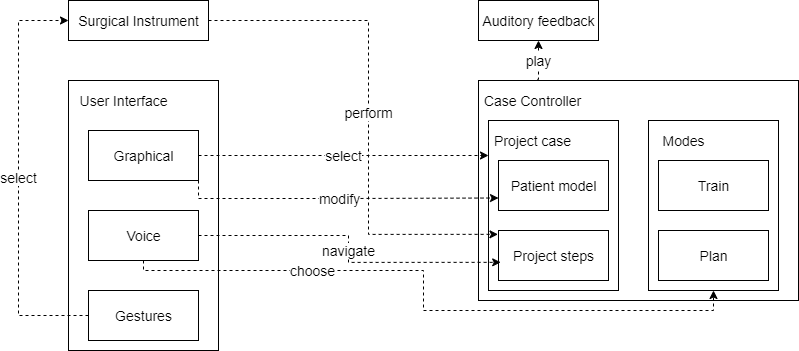
\includegraphics[width=375px]{images/implementation/architecture.png}
    \caption{\label{fig::ImplementationArchitecture}High-level overview of the applications architecture. Interactions between system components are visualized.}
\end{figure}

The broad overview of how individual system components interact with each other is depicted in Figure \ref{fig::ImplementationArchitecture}.
The CaseController component is responsible for handling all project case related information.
Via the GUI, users load a project case into the CaseController.
Inside of the CaseController, users can choose to switch the currently active mode via the VUI.
The mode will decide how steps, which are added by the user via the currently selected surgical instrument, are handled inside of the CaseController.
In planning mode, steps are directly added to the project case, while in training mode the correct execution of the procedure will be checked.
Either way, the CaseController calls the Auditory Feedback component to play auditory confirmations or errors to the user.
Surgical instruments are abstracted in such a way, that it does not matter which instrument is currently selected.
New steps get passed to the CaseController in form of a geometric representation of the procedure with a new material attached to it.

\section{\label{sec::VirtualOperatingRoom}Virtual Operating Room}
The related works highlight that presence of users, as shown by Pulijala et al. can effectively decrease trainees anxiety and stress before real operations \cite{Pulijala.2017}.
To increase the presence of users inside of VR \ref{req::F1}, a virtual operating room has been designed with photogrammetry.

\begin{figure}[ht]
    \centering
    \begin{minipage}{.5\textwidth}
      \centering
      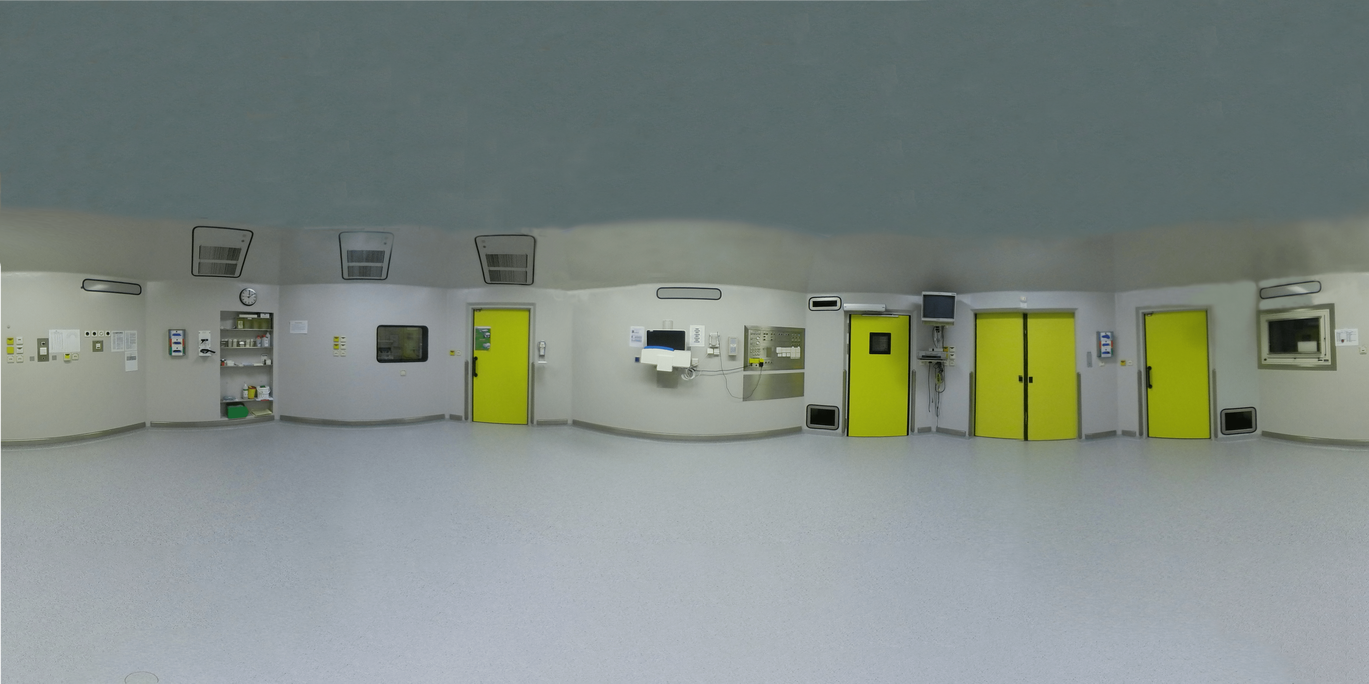
\includegraphics[width=0.99\linewidth]{images/implementation/vot/operating_room_360.png}
    \end{minipage}%
    \begin{minipage}{.5\textwidth}
      \centering
      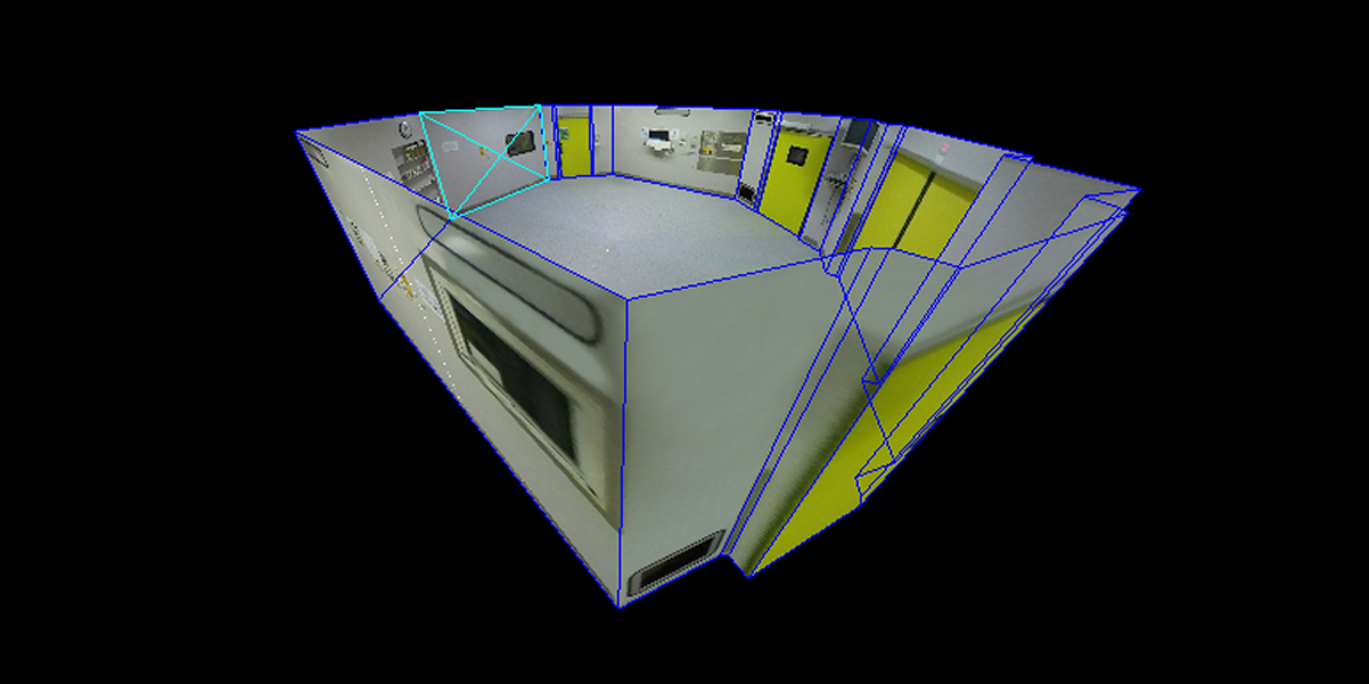
\includegraphics[width=0.99\linewidth]{images/implementation/vot/walkabout_worlds.png}
    \end{minipage}
    \caption{\label{fig::360OperatingRoom}Left: Edited 360 Degree Photograph of an OT in UHA. Right: Result of conversion to 3D model via Walkabout Worlds}
\end{figure}

The virtual operating room has been modeled with a cost-effective, simplistic photogrammatry-esque approach, in which a real operation room from UHA has been captured using a 
360-degree camera (Figure \ref{fig::360OperatingRoom}), the Samsung Gear 360, and converted into a 3D model via Walkabout Worlds \cite{WalkaboutWorlds}.
For reference, the operating room 10 from UHA Aachen has been caputured and modeled for use in VR.
Beforehand, the operating room was emptied out as much as possible and then, after converting it to a 3D model, filled with freely avaliable 3D objects from open assets in Unity3D.
This way, users can feel present inside of a real OT while being able to interact with any subsequently imported 3D models found in the surgical environment.
Some details, such as the operating table dock in the middle of the room have been edited out with photo-editing software.
Note that any operating room can be modeled and added to the existing application (Requirement \ref{req::N8}).


\begin{figure}[ht]
  \centering
  \begin{minipage}{.5\textwidth}
    \centering
    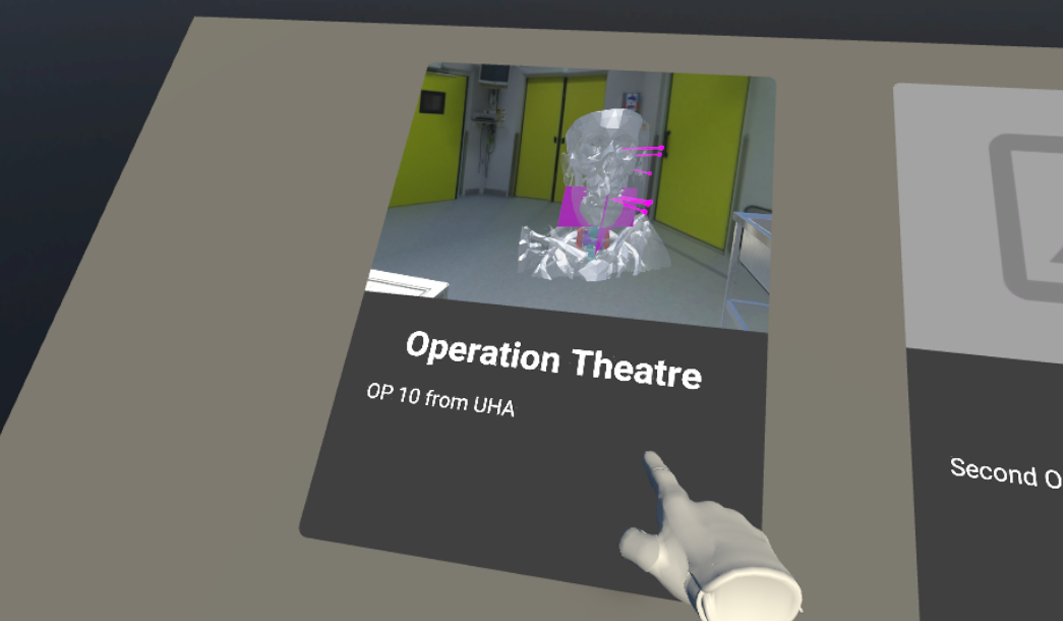
\includegraphics[width=0.99\linewidth, height=5.1cm]{images/implementation/vot/select_op.png}
  \end{minipage}%
  \begin{minipage}{.5\textwidth}
    \centering
    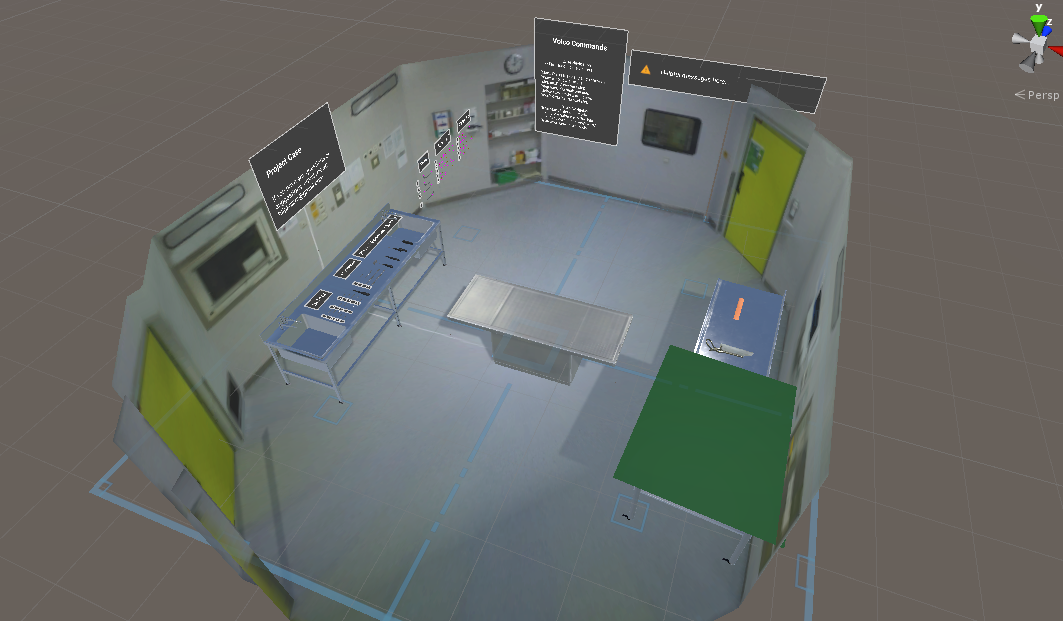
\includegraphics[width=0.99\linewidth, height=5.1cm]{images/implementation/vot/overview.png}
  \end{minipage}
  \caption{\label{fig::SceneSelect} Left: Users choose which OT they want to work in by selecting the thumbnail of an OT with their virtual hands. Right: The final virtual OT for OMFS. 
  The OT table with the patient is located in the middle. Next to it, a tray with surgical instruments.
  Textual information relevant to the procedure is floating next to the operating table.}
\end{figure}

Users can choose which OT they want to work in by selecting it in the OT select view (Figure \ref{fig::SceneSelect}).
The OT, which was created for this thesis consists of an instrument tray, where all instruments are located including their descriptive labels, the operating table, and two smaller trays 
for placing used instruments.
Additionally, information relevant to the project case is displayed inside of the OT as depicted in Figure \ref{fig::SceneSelect}.
\\ Surgical instruments were scanned via medical imaging acquisition and postprocessed in Blender3D to reduce artifacts, which occur during the 3D scanning phase of the surgical instruments and materials.
After these critical steps for immersion and presence (especially for the OMF surgeons of UHA) have been completed, instruments and materials are ready to be imported into Unity3D.
Users navigate through the OT via the locomotion options (Figure \ref{sec::Architecture}), and interact with the environment via a combination of natural gestures, GUI and VUI, as will be discussed 
extensively in the following Section.
\\ In principle, users can create their own OT and surgical instruments specialized to their medical field, import them into Unity3D, and the underlying architecture (Figure \ref{sec::Architecture}) 
will continue to work.
\section{\label{sec::UserInterface}User Interface}
At this point, the aforementioned six procedures are implemented in the system.
However, as described in Section \ref{sec::Architecture}, the system is extensible in the regard that new instruments can be implemented.
Currently, the implemented instruments are based on the workflow of OMF surgeons of the UHA: Users can perform drilling, hammer and chisel, bonesaw and milling operations.
Additionally, users can place markings and osteosynthesis plates on the virtual patient.
\\ To perform procedures, a project case has to be loaded first, as described in Section \ref{sec::GraphicalUserInterface}.
In the sense of SteamVRs interaction system described in Section \ref{sec::Architecture}, for each procedure there is an 'indicate' action when the user touches the 'perform' button, as well as an 'perform' action when the user presses the button all the way.
This way, users get a visual feedback when they are about to perform a procedure, as well as having visual indications of where the procedure will start (i.e. tip of the surgical instrument).
After described each procedure individually, how the procedures come together to create the steps for a procedure will be shortly desctribed.
\\ Each procedure will add a step to the project case.
In the sense of the VR-AR-based workflow described in Section \ref{sec::Workflow}, project cases can then be loaded into both parts of the workflow.
The steps are added to the hierarchy of the patient's 3D model and are identified as a step by name.
Through using this kind of approach, extensibility is guaranteed as each new instrument simply has to add some kind of geometry as a step to the project case (Requirements \ref{req::N8}, \ref{req::F3.7}).
It follows that any kind of procedure can then be imported into the AR workflow, even without touching the application.
\\ When a procedure is performed, users get voice feedback confirming that a step has been added to the project case.
Users can also navigate the project cases steps by using the VUIs commands, so that navigation through the steps of the procedure can be done while holding surgical instruments (Requirements \ref{req::N1}, \ref{req::F3.7}).
\\ For some of the surgical instruments, the user representation of the hand will be shown, for others not.
When a surgical instrument has this feature implemented, it is guaranteed that the instrument will always be grabbed and positioned in the same position on the hand, meaning the handgrip will always be the same.
However, in some cases, f.e. sawing with the bonesaw, this feature would prevent users from switching the handgrip of the surgical instrument. 
Therefore, for some instruments, this feature was removed.
Users will not see their virtual hands on the surgical instrument, but can chose to hold it however they want.
The virtual hands will be hidden while holding the instrument, however the instrument still represents the users hand position.
This way, the handgrip of the instrument can be adapted as users see fit.
The decision, on which was decided if hands should be hidden when grabbing an instrument, was made by a trial and error approach with the help of a physician's opinion on whether this features was useful.
The procedure specific implementation will be thoroughly described in the following.

\paragraph{Drilling}

The \textbf{drilling} operation is performed by first picking up the drill handle from the instrument tray via the grabbing action (Figure \ref{fig::FeatureDrillingAttachments}).
Since drills are typically held in a number of different ways, the handgrip of the drill handle is adjustable.
Therefore, the virtual hand will not be displayed while holding the drill.
The instrument tray is located next to the operating table, where the patient's model will initially be positioned.
The drill handle initially has no attachment; users have to attach a drill bit first.

\begin{figure}[ht]
    \centering
    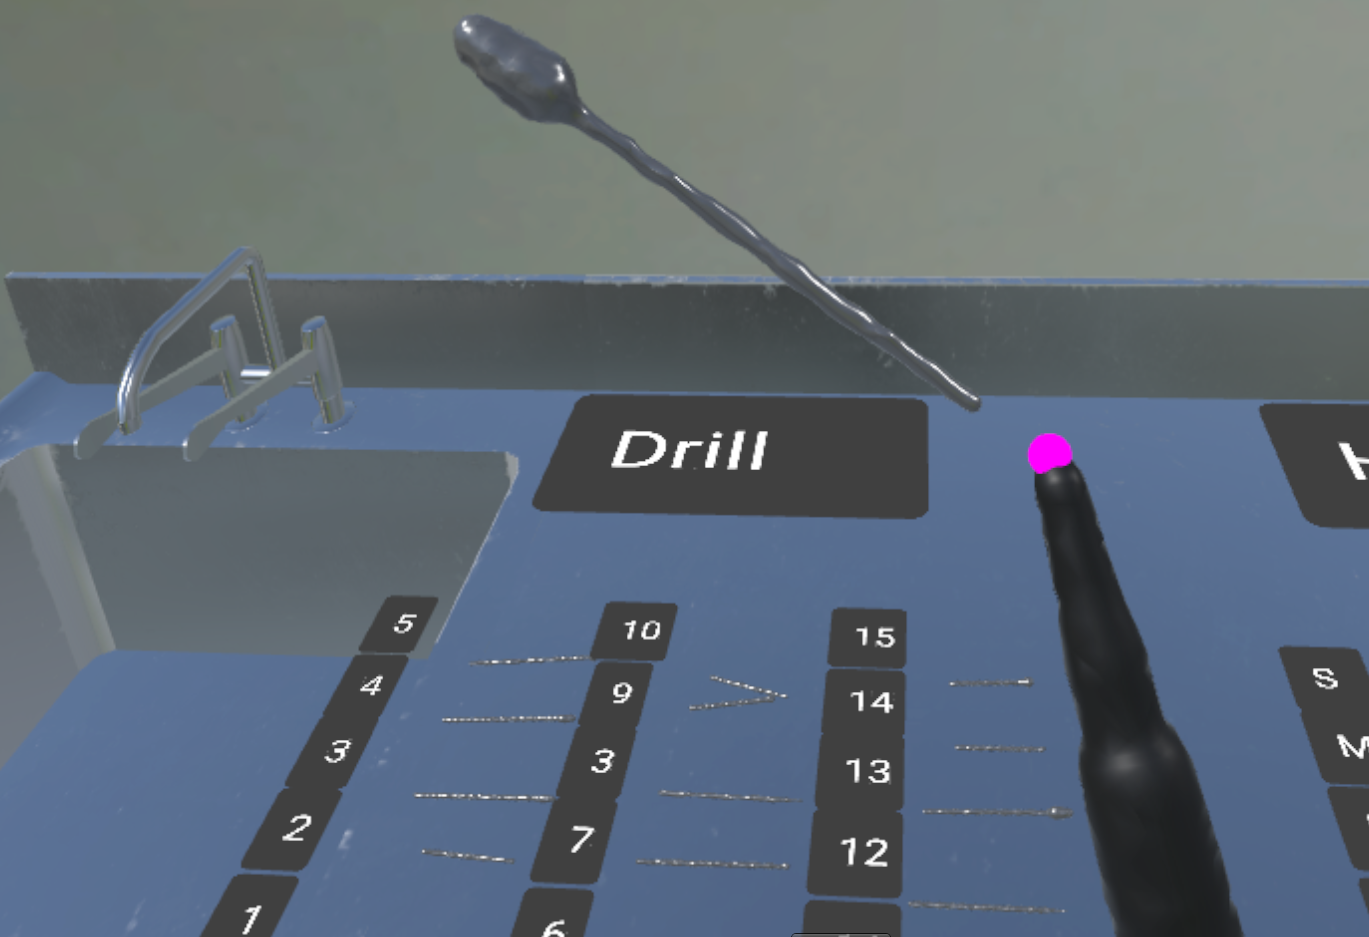
\includegraphics[width=200px]{images/implementation/features/procedures/drilling_attachment.png}
    \caption{\label{fig::FeatureDrillingAttachments}Process of attaching drill bit to the drill handle. With the right hand, the user performs the indicate action by touching 
    the respective button. With the other hand, the bit is picked up by grabbing it and moved into the pink sphere to attach the attachment.}
\end{figure}

In total, there are fifteen bits which can be used as an attachment for the drilling procedure.
Bits are modeled after their real counterparts in UHA.
They differ in size, length and width.
A visual signal is shown to the user while the indicate action is performed on the hand holding the drill handle.
By moving a drill bit to the visual indicator, the bit is attached to the handle (Figure \ref{fig::FeatureDrillingAttachments}).
Swapping out bits is performed by simply moving another bit into the indicator.
To perform the procedure, the drill handle must have a bit attached. 

\begin{figure}[ht]
    \centering
    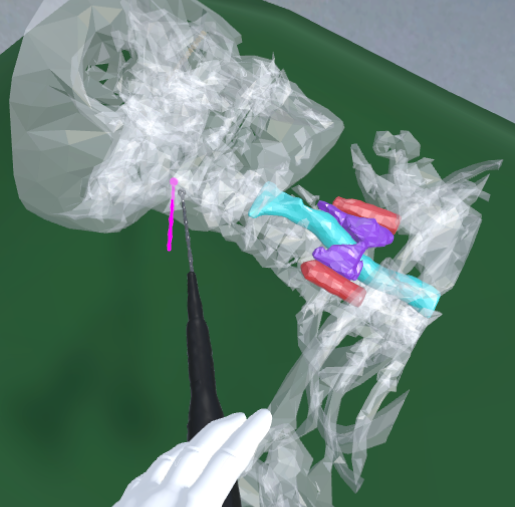
\includegraphics[width=200px]{images/implementation/features/procedures/drilling.png}
    \caption{\label{fig::FeatureDrilling}Drilling procedure. The pink object represents the last performed step, which was performed using the currently selected tool by pressing 
    the respective button all the way.}
\end{figure}

By triggering the perform action of the hand holding the drill, a copy of the currently attached drill bit is created and added to the project case. 
This copy has a different material, i.e. a pink material, to indicate that it is part of the project case (Figure \ref{fig::FeatureDrilling}).
Additionally, textual information about the currently attached drill bit will be stored in the project case, so that the exact procedure can be reproduced later (Requirements \ref{req::N3}, \ref{req::N5}).
The drill bit will not be removed on performing a procedure, so that multiple drilling steps can be performed consecutively.
When the drill is no longer needed, it can either be placed back on the instrument tray or the operating table for quick access.
Note that any instrument, excluding the osteosynthesis plates described later, can be placed anywhere in the OT.
\paragraph{Chiseling}

The \textbf{chiseling} procedure has two parts to it.
First, with one hand a chisel has to be chosen.
Users have a choice between a small, medium, large and extra large chisel to perform the procedure.
With the other hand, users then have to pick up the hammer.
Since this procedure requires users to hold two surgical instruments at the same time, this procedure can get cumbersome.
However, users can easily avoid this by placing the instruments on the operating table in the middle of the OT and repositioning afterwards (Figure \ref{fig::ChiselPrepare}).

\begin{figure}[ht]
    \centering
    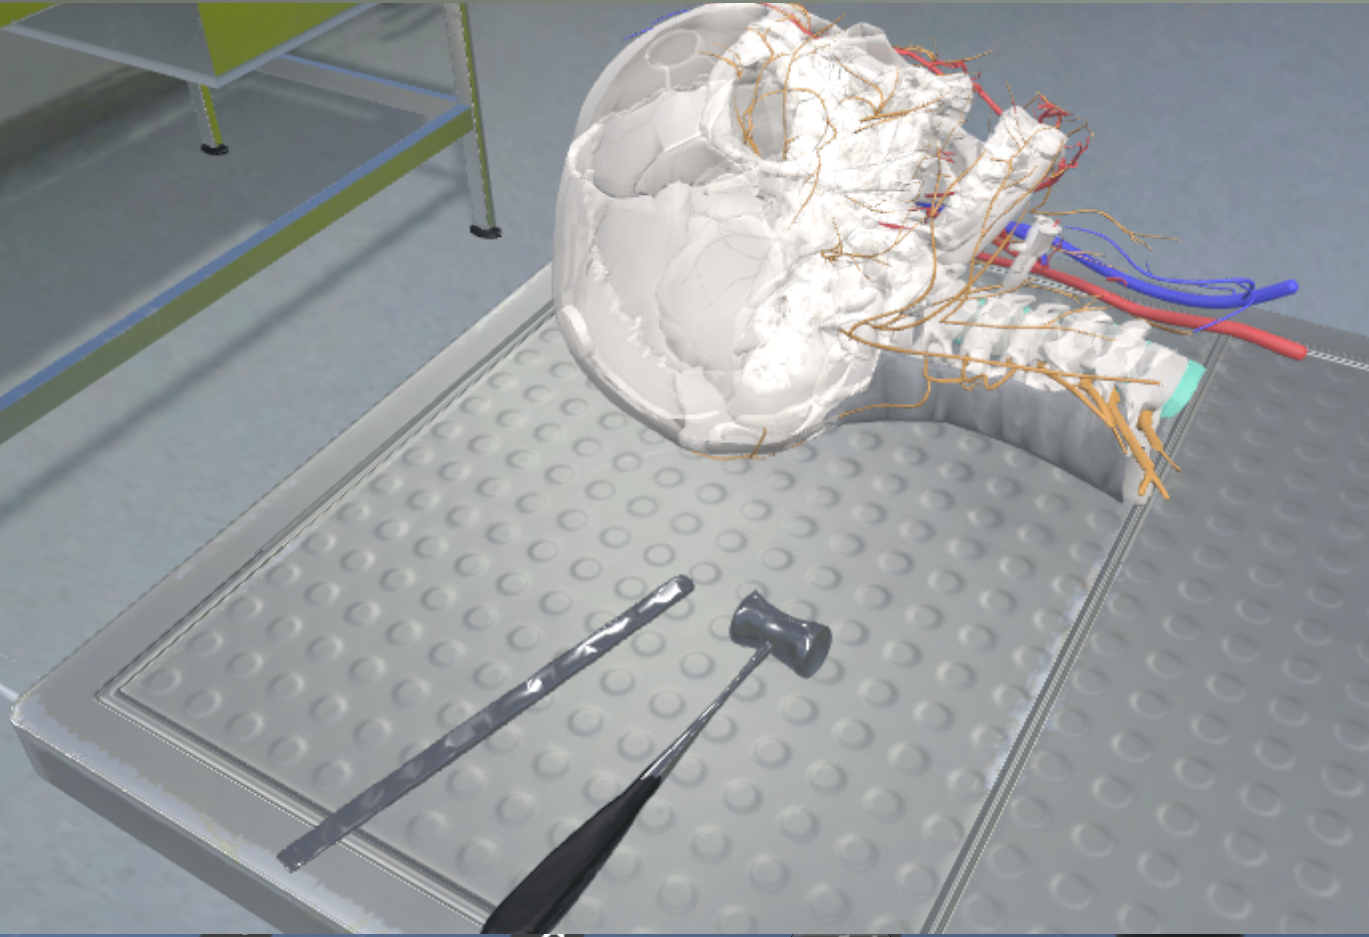
\includegraphics[width=\linewidth]{images/implementation/features/procedures/chisel_prepare.png}
    \caption{\label{fig::ChiselPrepare}The user prepares for the chiseling procedure by placing the instruments on the OT where the patient is located.
    indicators with the hammer in the other hand to perform the procedure.}
\end{figure}

When users have the perfect viewpoint, they can take up both instruments once again and start the procedure.
By pressing the indicate button on the hand where the chisel is located, rectangular indications at the top and bottom end of the chisel are shown to the user.
While these indications are active, the user has to perform a hammering motion with the hand holding the hammer.

\begin{figure}[ht]
    \centering
    \begin{minipage}{.5\textwidth}
      \centering
      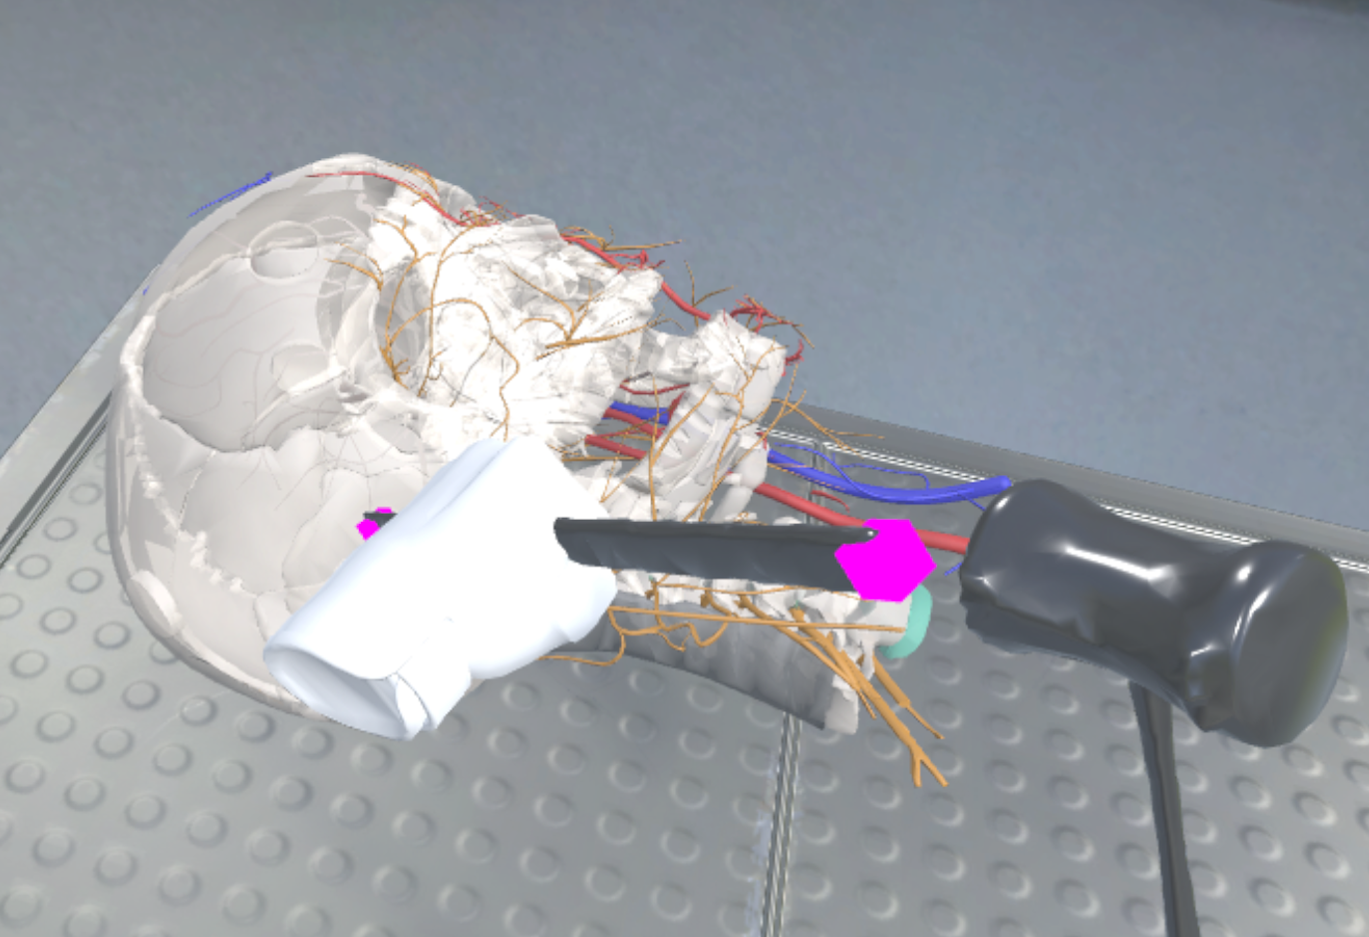
\includegraphics[width=0.99\linewidth]{images/implementation/features/procedures/chisel_1.png}
    \end{minipage}%
    \begin{minipage}{.5\textwidth}
      \centering
      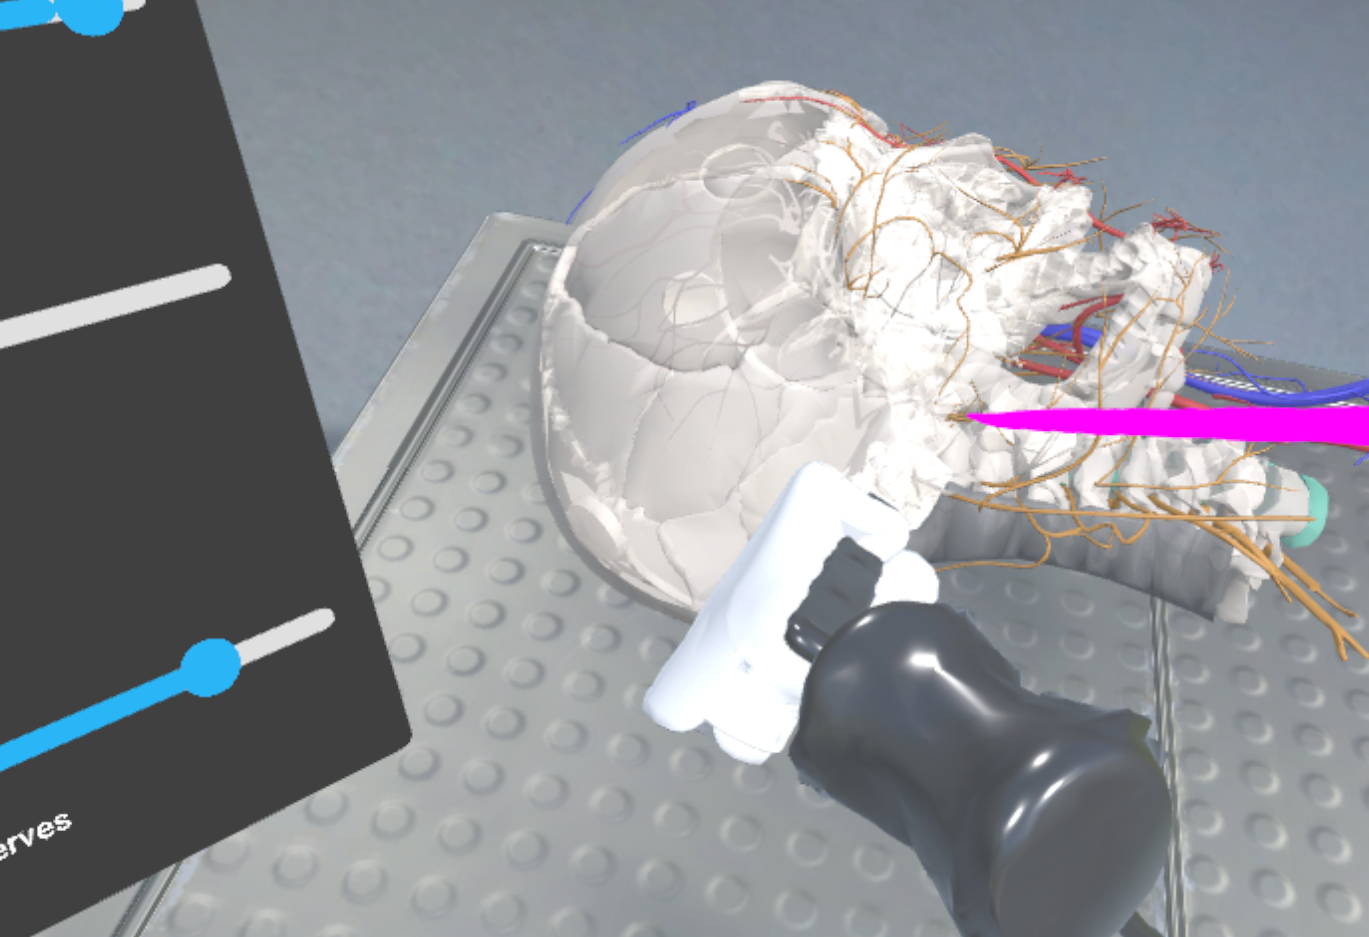
\includegraphics[width=0.99\linewidth]{images/implementation/features/procedures/chisel_2.png}
    \end{minipage}
    \caption{\label{fig::ChiselProcedure}Process of the chiseling procedure. Left: The users uses the indicate action with his left hand in preparation for the procedure. Right: After hammering on the indication on the chisel, the procedure has been performed and a step is generated.}
\end{figure}

When they hit the rectangular indicators located on the chisel, the chiseling procedure step is added to the project case in form of a modified copy of the hold chisel (Figure \ref{fig::ChiselProcedure}).
Here, information about the performed step is also included in the form of chisel size used for the procedure. 
\paragraph{Sawing}

\begin{figure}[ht]
    \centering
    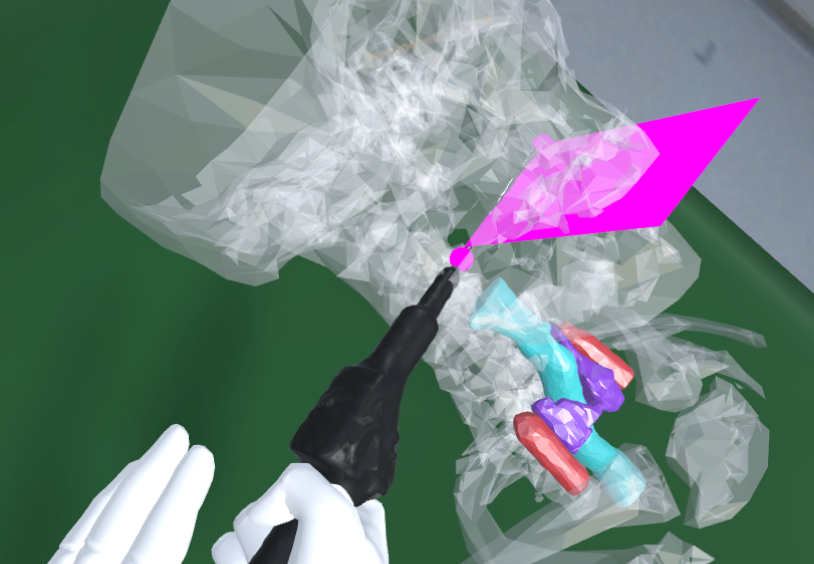
\includegraphics[width=200px]{images/implementation/features/procedures/bonesaw.png}
    \caption{\label{fig::FeatureBoneSaw}Bonesaw Procedure}
\end{figure}

The \textbf{sawing} procedure is performed by picking up the bonesaw.
Touch the controller will show two indications to the user (Figure \ref{fig::FeatureBoneSaw}).
The procedure is performed by first pressing down the trigger button and then letting go of it.
When letting go of the trigger button, a two dimensianal plane is created in the three dimensional space by using four points.
Two of these points are created when pressing down, and the other two when letting go of the trigger button.
A plane is then created with which the user can reproduce the way in which the bonesaw has been moved.
Arbitrary cutting shapes can be created by breaking them down into two-dimensional shapes and performing multiple movements.
\paragraph{Milling}

\begin{figure}[ht]
    \centering
    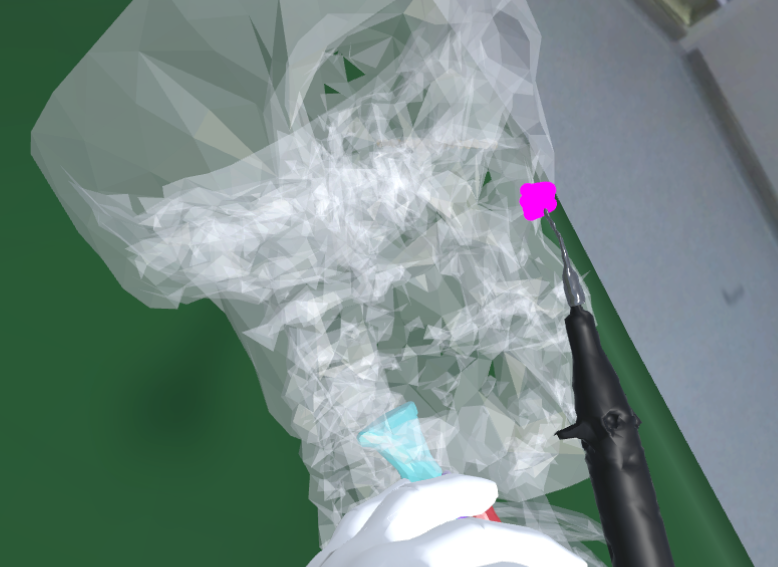
\includegraphics[width=200px]{images/implementation/features/procedures/piezo.png}
    \caption{\label{fig::FeaturePiezo}Milling procedure. Holding down the trigger button will draw little spheres until the button is released. The resulting object represents the volumetric space which is to be milled.}
\end{figure}

The \textbf{milling} operation is performed by grabbing the piezo instrument.
The indicator for the piezo is at the tip of the instrument, indicating which area will be milled.
While the "perform" button is being held down, little spheres are being drawn at the tip of the instrument \ref{fig::FeaturePiezo}.
When the button is released, the shapes are combined into a single 3D model and added as a project step.
The resulting object represents the volumetric space which has to be milled in the procedure.
The procedure can be reconstructed by "milling" the same 3D space in the virtual operating room.
\begin{figure}[ht!]
    \centering
    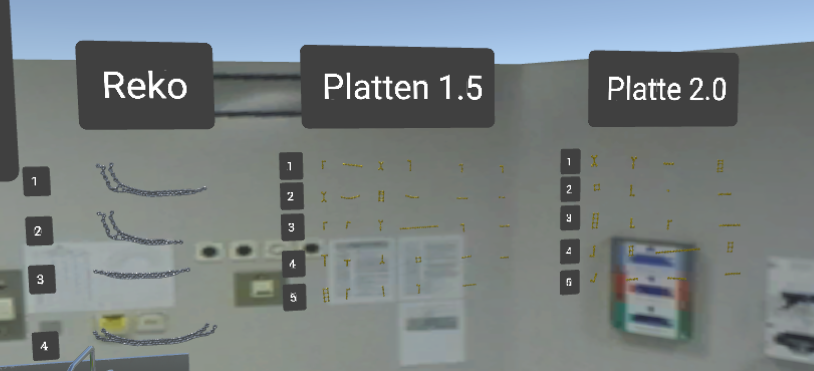
\includegraphics[width=\linewidth]{images/implementation/features/procedures/metal_plates_1.png}
    \caption{\label{fig::FeatureMetalPlate} Osteosynthesis Plates Overview}
\end{figure}

The osteosynthesis plates procedure consists of two steps before adding it as a step to the project case.
First, users have to chose which plate to use (Figure \ref{fig::FeatureMetalPlate}).
The user can chose from four reconstruction plates, 29 1.5mm plates and 20 2.0mm plates (Firma Angeben, osteosynthesis plates).
The optimal plates to use vary due to the pathology of the patient and the previously performed procedures.
After selecting the proper plate, a number of indicators will show to the user (Figure \ref{fig::FeatureMetalPlate2}).
In the context of the osteosynthesis plates, these indicators are "control points", with which the user can bend and twist the plates.
Bending and twisting is performed by chosing a control point via hovering them with the users free hand and grabbing them.
Then, the user has to translate and rotate the control point in the desired manner.
\begin{figure}
  \centering
  \begin{minipage}{.5\textwidth}
    \centering
    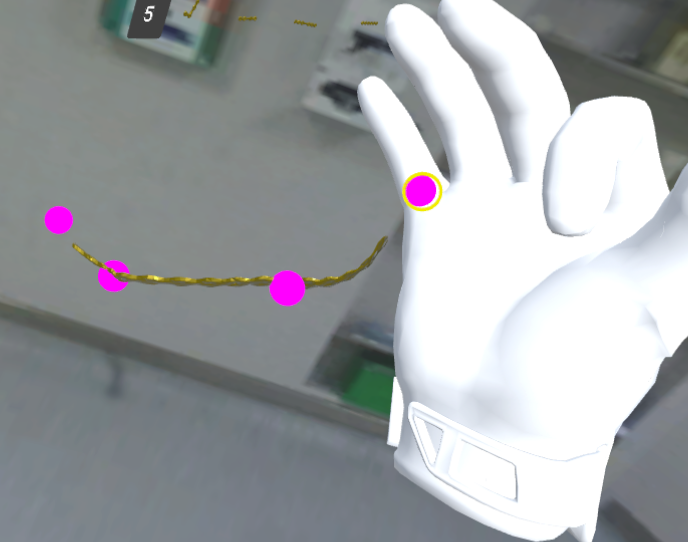
\includegraphics[width=0.95\linewidth]{images/implementation/features/procedures/metal_plates_2.png}
  \end{minipage}%
  \begin{minipage}{.5\textwidth}
    \centering
    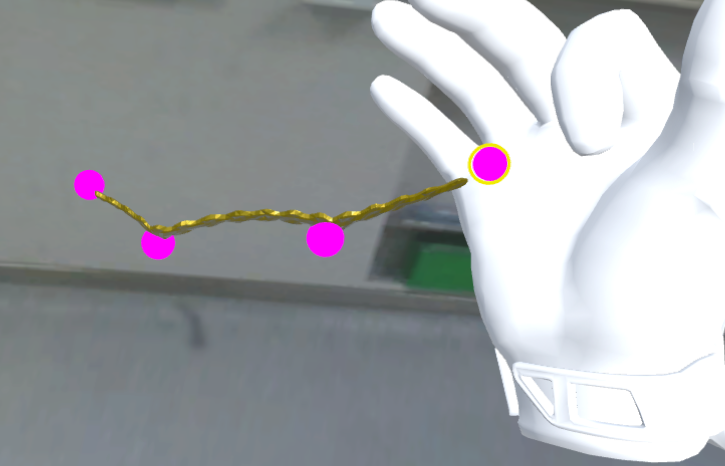
\includegraphics[width=0.95\linewidth]{images/implementation/features/procedures/metal_plates_3.png}
  \end{minipage}
  \caption{\label{fig::FeatureMetalPlate2}Osteosynthesis Plates Modifications. User can translate and rotate "control points" to perform modifications to the plates shape} 
\end{figure}

The user can then observe in which way this has affected the shape of the metal plate and either position the plate on the patient or perform more modifications to the plates via controlpoints.
The correct modification of the metal plates differs quite a lot from real life modifications to the plates.
However even though there is a slight learning curve to it, the modification is consistent and predictable (Figure \ref{fig::FeatureMetalPlate2}).


\begin{figure}[ht!]
    \centering
    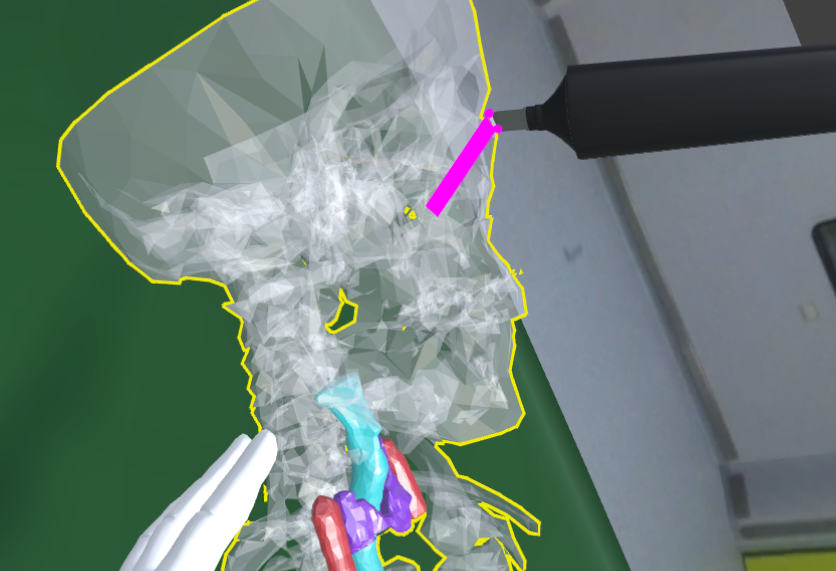
\includegraphics[width=\linewidth]{images/implementation/features/procedures/marker.png}
    \caption{\label{fig::FeatureMarker}Marker Procedure}
\end{figure}

The marking procedure is similar to the bonesaw procedure, meaning that rectangular shapes are drawed into the three dimensianal space (Figure \ref{fig::FeatureMarker}).
However, here the created shapes are much thinner.
In contrast to the bonesaw, the virtual hands of the user are also disabled here.
This way, the user can decide to hold the marker in the optimal way.
Since the main objective is marking specific spots on the patient, this is the natural approach.
\section{\label{sec::Features}Features}
At this point, the aforementioned six procedures are implemented in the system.
However, as described in Section \ref{sec::Architecture}, the system is extensible in the regard that new instruments can be implemented.
Currently, the implemented instruments are based on the workflow of OMF surgeons of the UHA: Users can perform drilling, hammer and chisel, bonesaw and milling operations.
Additionally, users can place markings and osteosynthesis plates on the virtual patient.
\\ To perform procedures, a project case has to be loaded first, as described in Section \ref{sec::GraphicalUserInterface}.
In the sense of SteamVRs interaction system described in Section \ref{sec::Architecture}, for each procedure there is an 'indicate' action when the user touches the 'perform' button, as well as an 'perform' action when the user presses the button all the way.
This way, users get a visual feedback when they are about to perform a procedure, as well as having visual indications of where the procedure will start (i.e. tip of the surgical instrument).
After described each procedure individually, how the procedures come together to create the steps for a procedure will be shortly desctribed.
\\ Each procedure will add a step to the project case.
In the sense of the VR-AR-based workflow described in Section \ref{sec::Workflow}, project cases can then be loaded into both parts of the workflow.
The steps are added to the hierarchy of the patient's 3D model and are identified as a step by name.
Through using this kind of approach, extensibility is guaranteed as each new instrument simply has to add some kind of geometry as a step to the project case (Requirements \ref{req::N8}, \ref{req::F3.7}).
It follows that any kind of procedure can then be imported into the AR workflow, even without touching the application.
\\ When a procedure is performed, users get voice feedback confirming that a step has been added to the project case.
Users can also navigate the project cases steps by using the VUIs commands, so that navigation through the steps of the procedure can be done while holding surgical instruments (Requirements \ref{req::N1}, \ref{req::F3.7}).
\\ For some of the surgical instruments, the user representation of the hand will be shown, for others not.
When a surgical instrument has this feature implemented, it is guaranteed that the instrument will always be grabbed and positioned in the same position on the hand, meaning the handgrip will always be the same.
However, in some cases, f.e. sawing with the bonesaw, this feature would prevent users from switching the handgrip of the surgical instrument. 
Therefore, for some instruments, this feature was removed.
Users will not see their virtual hands on the surgical instrument, but can chose to hold it however they want.
The virtual hands will be hidden while holding the instrument, however the instrument still represents the users hand position.
This way, the handgrip of the instrument can be adapted as users see fit.
The decision, on which was decided if hands should be hidden when grabbing an instrument, was made by a trial and error approach with the help of a physician's opinion on whether this features was useful.
The procedure specific implementation will be thoroughly described in the following.

\paragraph{Drilling}

The \textbf{drilling} operation is performed by first picking up the drill handle from the instrument tray via the grabbing action (Figure \ref{fig::FeatureDrillingAttachments}).
Since drills are typically held in a number of different ways, the handgrip of the drill handle is adjustable.
Therefore, the virtual hand will not be displayed while holding the drill.
The instrument tray is located next to the operating table, where the patient's model will initially be positioned.
The drill handle initially has no attachment; users have to attach a drill bit first.

\begin{figure}[ht]
    \centering
    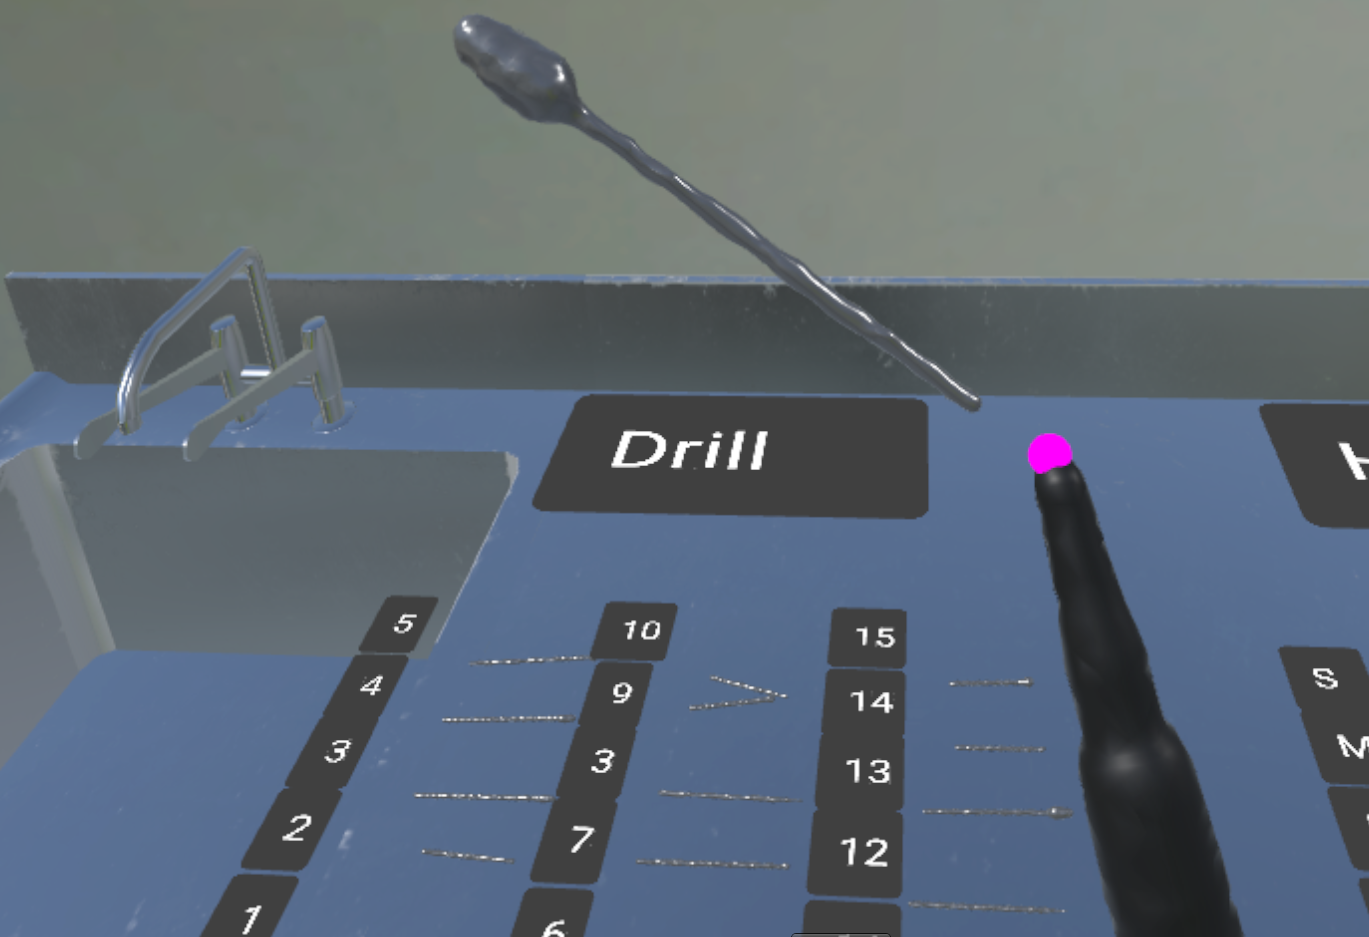
\includegraphics[width=200px]{images/implementation/features/procedures/drilling_attachment.png}
    \caption{\label{fig::FeatureDrillingAttachments}Process of attaching drill bit to the drill handle. With the right hand, the user performs the indicate action by touching 
    the respective button. With the other hand, the bit is picked up by grabbing it and moved into the pink sphere to attach the attachment.}
\end{figure}

In total, there are fifteen bits which can be used as an attachment for the drilling procedure.
Bits are modeled after their real counterparts in UHA.
They differ in size, length and width.
A visual signal is shown to the user while the indicate action is performed on the hand holding the drill handle.
By moving a drill bit to the visual indicator, the bit is attached to the handle (Figure \ref{fig::FeatureDrillingAttachments}).
Swapping out bits is performed by simply moving another bit into the indicator.
To perform the procedure, the drill handle must have a bit attached. 

\begin{figure}[ht]
    \centering
    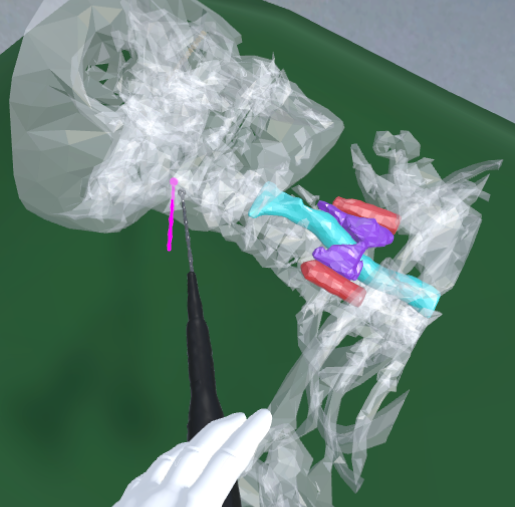
\includegraphics[width=200px]{images/implementation/features/procedures/drilling.png}
    \caption{\label{fig::FeatureDrilling}Drilling procedure. The pink object represents the last performed step, which was performed using the currently selected tool by pressing 
    the respective button all the way.}
\end{figure}

By triggering the perform action of the hand holding the drill, a copy of the currently attached drill bit is created and added to the project case. 
This copy has a different material, i.e. a pink material, to indicate that it is part of the project case (Figure \ref{fig::FeatureDrilling}).
Additionally, textual information about the currently attached drill bit will be stored in the project case, so that the exact procedure can be reproduced later (Requirements \ref{req::N3}, \ref{req::N5}).
The drill bit will not be removed on performing a procedure, so that multiple drilling steps can be performed consecutively.
When the drill is no longer needed, it can either be placed back on the instrument tray or the operating table for quick access.
Note that any instrument, excluding the osteosynthesis plates described later, can be placed anywhere in the OT.
\paragraph{Chiseling}

The \textbf{chiseling} procedure has two parts to it.
First, with one hand a chisel has to be chosen.
Users have a choice between a small, medium, large and extra large chisel to perform the procedure.
With the other hand, users then have to pick up the hammer.
Since this procedure requires users to hold two surgical instruments at the same time, this procedure can get cumbersome.
However, users can easily avoid this by placing the instruments on the operating table in the middle of the OT and repositioning afterwards (Figure \ref{fig::ChiselPrepare}).

\begin{figure}[ht]
    \centering
    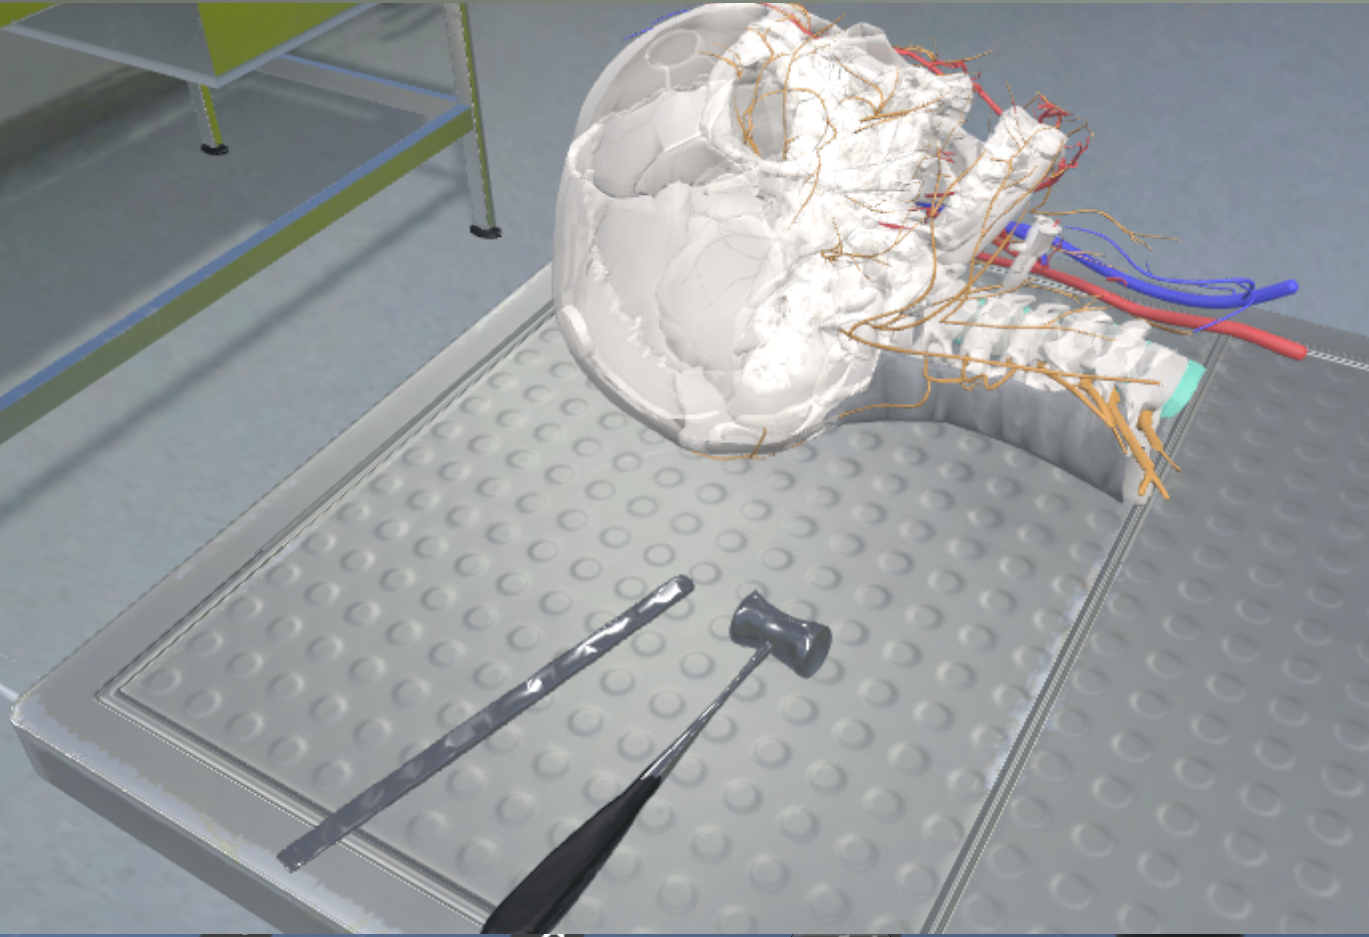
\includegraphics[width=\linewidth]{images/implementation/features/procedures/chisel_prepare.png}
    \caption{\label{fig::ChiselPrepare}The user prepares for the chiseling procedure by placing the instruments on the OT where the patient is located.
    indicators with the hammer in the other hand to perform the procedure.}
\end{figure}

When users have the perfect viewpoint, they can take up both instruments once again and start the procedure.
By pressing the indicate button on the hand where the chisel is located, rectangular indications at the top and bottom end of the chisel are shown to the user.
While these indications are active, the user has to perform a hammering motion with the hand holding the hammer.

\begin{figure}[ht]
    \centering
    \begin{minipage}{.5\textwidth}
      \centering
      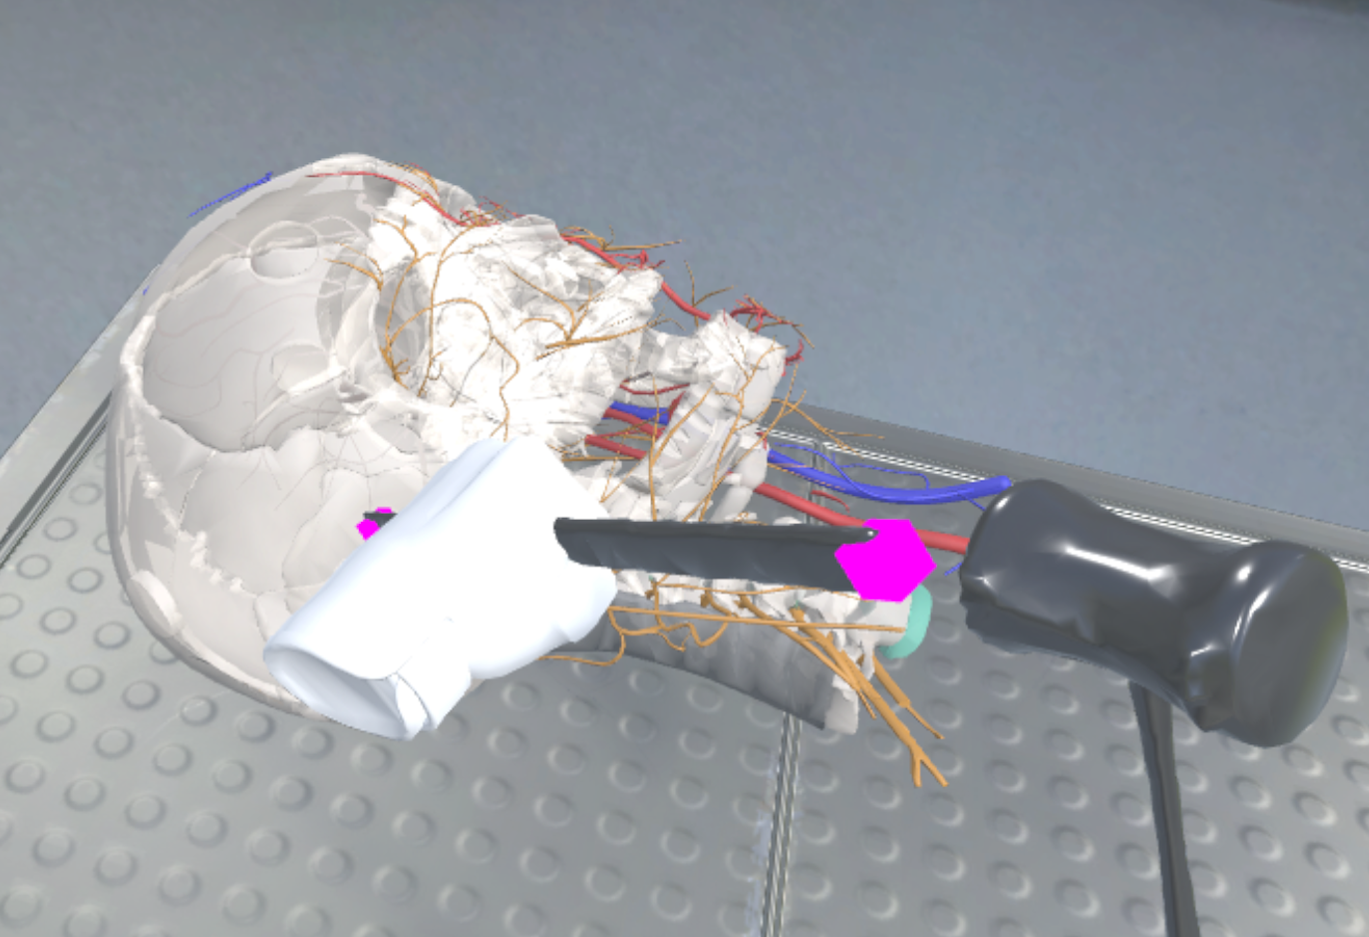
\includegraphics[width=0.99\linewidth]{images/implementation/features/procedures/chisel_1.png}
    \end{minipage}%
    \begin{minipage}{.5\textwidth}
      \centering
      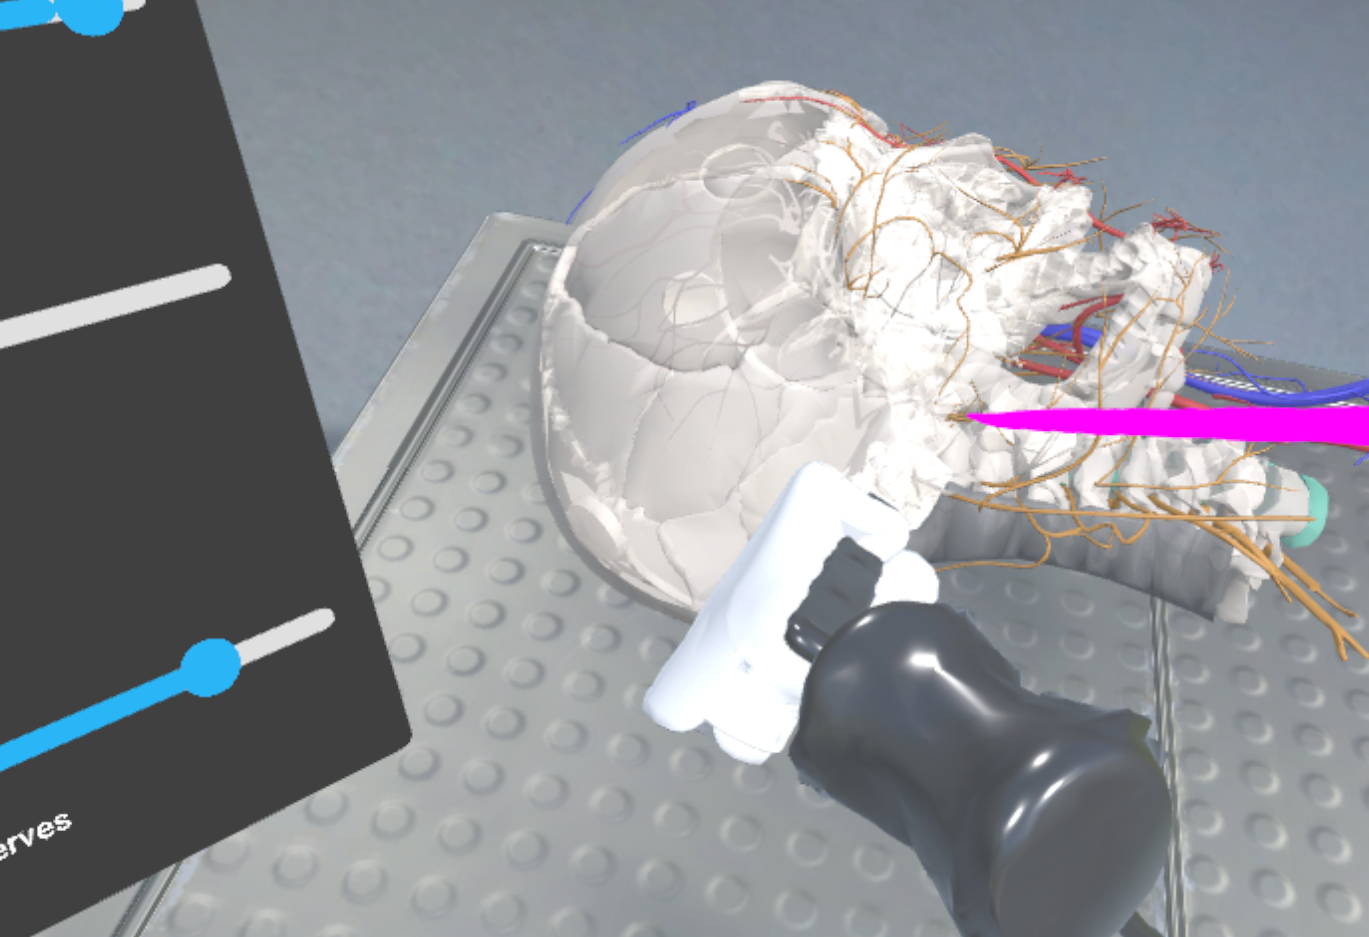
\includegraphics[width=0.99\linewidth]{images/implementation/features/procedures/chisel_2.png}
    \end{minipage}
    \caption{\label{fig::ChiselProcedure}Process of the chiseling procedure. Left: The users uses the indicate action with his left hand in preparation for the procedure. Right: After hammering on the indication on the chisel, the procedure has been performed and a step is generated.}
\end{figure}

When they hit the rectangular indicators located on the chisel, the chiseling procedure step is added to the project case in form of a modified copy of the hold chisel (Figure \ref{fig::ChiselProcedure}).
Here, information about the performed step is also included in the form of chisel size used for the procedure. 
\paragraph{Sawing}

\begin{figure}[ht]
    \centering
    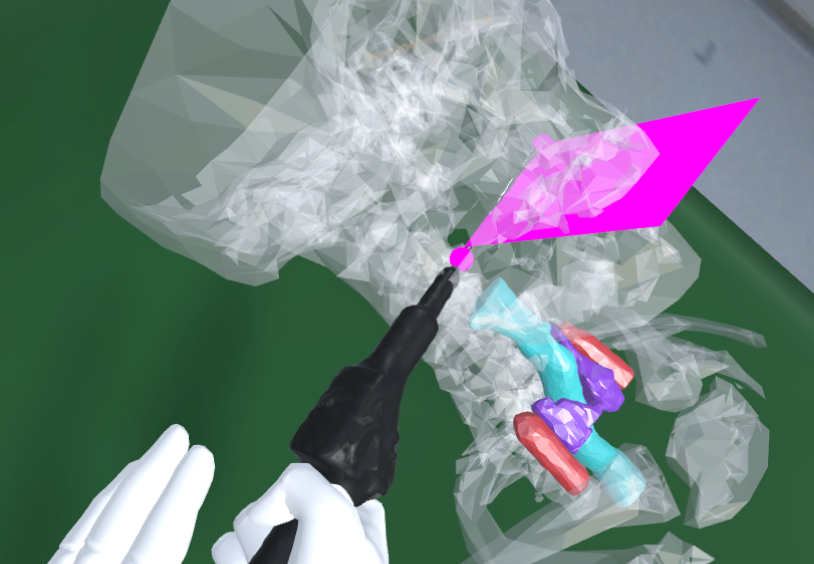
\includegraphics[width=200px]{images/implementation/features/procedures/bonesaw.png}
    \caption{\label{fig::FeatureBoneSaw}Bonesaw Procedure}
\end{figure}

The \textbf{sawing} procedure is performed by picking up the bonesaw.
Touch the controller will show two indications to the user (Figure \ref{fig::FeatureBoneSaw}).
The procedure is performed by first pressing down the trigger button and then letting go of it.
When letting go of the trigger button, a two dimensianal plane is created in the three dimensional space by using four points.
Two of these points are created when pressing down, and the other two when letting go of the trigger button.
A plane is then created with which the user can reproduce the way in which the bonesaw has been moved.
Arbitrary cutting shapes can be created by breaking them down into two-dimensional shapes and performing multiple movements.
\paragraph{Milling}

\begin{figure}[ht]
    \centering
    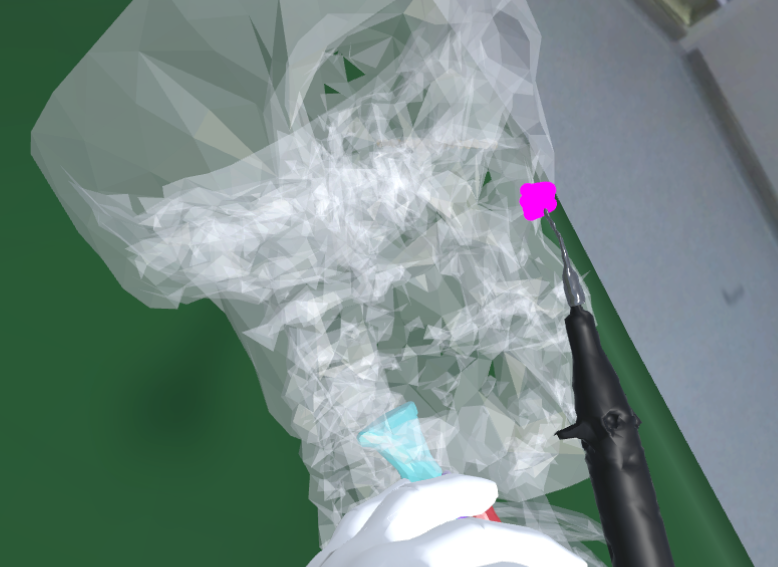
\includegraphics[width=200px]{images/implementation/features/procedures/piezo.png}
    \caption{\label{fig::FeaturePiezo}Milling procedure. Holding down the trigger button will draw little spheres until the button is released. The resulting object represents the volumetric space which is to be milled.}
\end{figure}

The \textbf{milling} operation is performed by grabbing the piezo instrument.
The indicator for the piezo is at the tip of the instrument, indicating which area will be milled.
While the "perform" button is being held down, little spheres are being drawn at the tip of the instrument \ref{fig::FeaturePiezo}.
When the button is released, the shapes are combined into a single 3D model and added as a project step.
The resulting object represents the volumetric space which has to be milled in the procedure.
The procedure can be reconstructed by "milling" the same 3D space in the virtual operating room.
\begin{figure}[ht!]
    \centering
    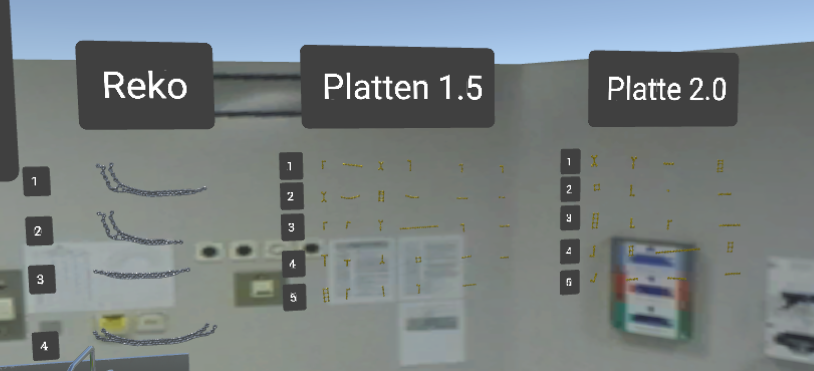
\includegraphics[width=\linewidth]{images/implementation/features/procedures/metal_plates_1.png}
    \caption{\label{fig::FeatureMetalPlate} Osteosynthesis Plates Overview}
\end{figure}

The osteosynthesis plates procedure consists of two steps before adding it as a step to the project case.
First, users have to chose which plate to use (Figure \ref{fig::FeatureMetalPlate}).
The user can chose from four reconstruction plates, 29 1.5mm plates and 20 2.0mm plates (Firma Angeben, osteosynthesis plates).
The optimal plates to use vary due to the pathology of the patient and the previously performed procedures.
After selecting the proper plate, a number of indicators will show to the user (Figure \ref{fig::FeatureMetalPlate2}).
In the context of the osteosynthesis plates, these indicators are "control points", with which the user can bend and twist the plates.
Bending and twisting is performed by chosing a control point via hovering them with the users free hand and grabbing them.
Then, the user has to translate and rotate the control point in the desired manner.
\begin{figure}
  \centering
  \begin{minipage}{.5\textwidth}
    \centering
    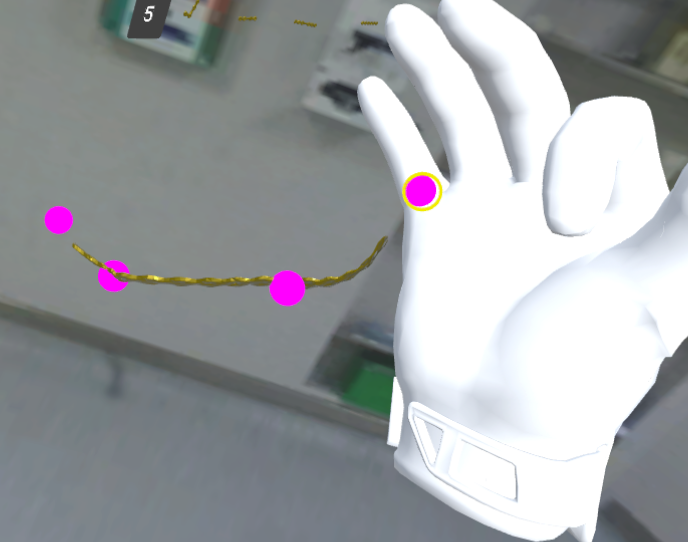
\includegraphics[width=0.95\linewidth]{images/implementation/features/procedures/metal_plates_2.png}
  \end{minipage}%
  \begin{minipage}{.5\textwidth}
    \centering
    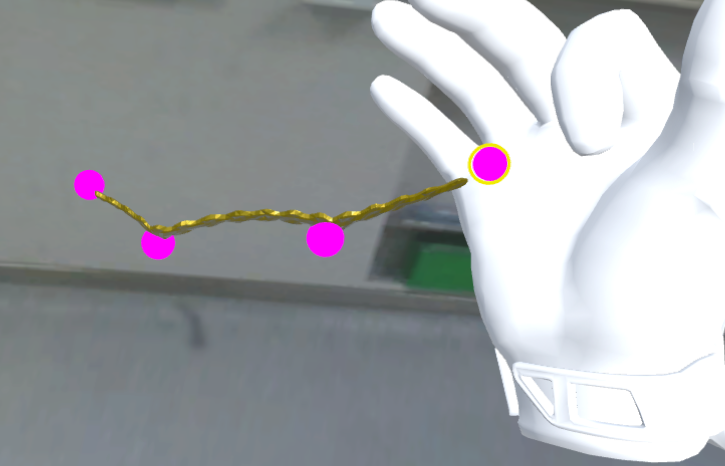
\includegraphics[width=0.95\linewidth]{images/implementation/features/procedures/metal_plates_3.png}
  \end{minipage}
  \caption{\label{fig::FeatureMetalPlate2}Osteosynthesis Plates Modifications. User can translate and rotate "control points" to perform modifications to the plates shape} 
\end{figure}

The user can then observe in which way this has affected the shape of the metal plate and either position the plate on the patient or perform more modifications to the plates via controlpoints.
The correct modification of the metal plates differs quite a lot from real life modifications to the plates.
However even though there is a slight learning curve to it, the modification is consistent and predictable (Figure \ref{fig::FeatureMetalPlate2}).


\begin{figure}[ht!]
    \centering
    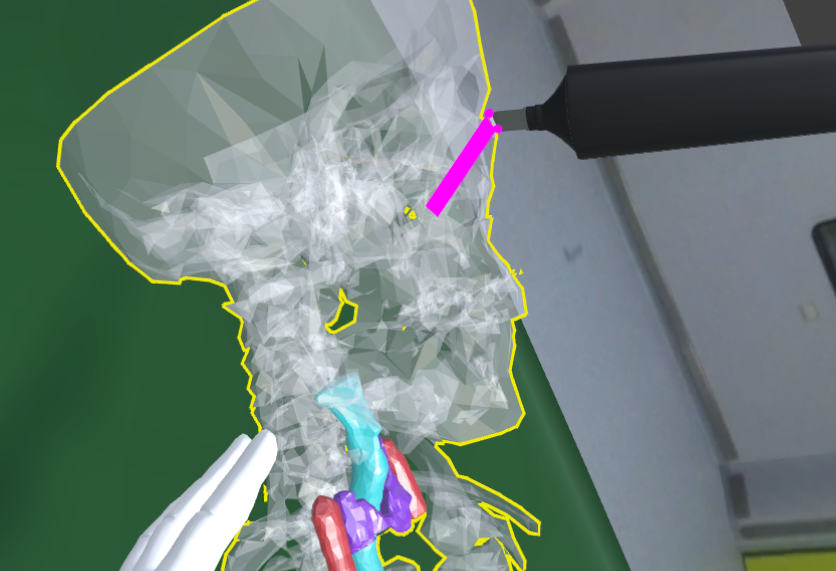
\includegraphics[width=\linewidth]{images/implementation/features/procedures/marker.png}
    \caption{\label{fig::FeatureMarker}Marker Procedure}
\end{figure}

The marking procedure is similar to the bonesaw procedure, meaning that rectangular shapes are drawed into the three dimensianal space (Figure \ref{fig::FeatureMarker}).
However, here the created shapes are much thinner.
In contrast to the bonesaw, the virtual hands of the user are also disabled here.
This way, the user can decide to hold the marker in the optimal way.
Since the main objective is marking specific spots on the patient, this is the natural approach.
\section{\label{sec::Workflow}Workflow}
At this point, the aforementioned six procedures are implemented in the system.
However, as described in Section \ref{sec::Architecture}, the system is extensible in the regard that new instruments can be implemented.
Currently, the implemented instruments are based on the workflow of OMF surgeons of the UHA: Users can perform drilling, hammer and chisel, bonesaw and milling operations.
Additionally, users can place markings and osteosynthesis plates on the virtual patient.
\\ To perform procedures, a project case has to be loaded first, as described in Section \ref{sec::GraphicalUserInterface}.
In the sense of SteamVRs interaction system described in Section \ref{sec::Architecture}, for each procedure there is an 'indicate' action when the user touches the 'perform' button, as well as an 'perform' action when the user presses the button all the way.
This way, users get a visual feedback when they are about to perform a procedure, as well as having visual indications of where the procedure will start (i.e. tip of the surgical instrument).
After described each procedure individually, how the procedures come together to create the steps for a procedure will be shortly desctribed.
\\ Each procedure will add a step to the project case.
In the sense of the VR-AR-based workflow described in Section \ref{sec::Workflow}, project cases can then be loaded into both parts of the workflow.
The steps are added to the hierarchy of the patient's 3D model and are identified as a step by name.
Through using this kind of approach, extensibility is guaranteed as each new instrument simply has to add some kind of geometry as a step to the project case (Requirements \ref{req::N8}, \ref{req::F3.7}).
It follows that any kind of procedure can then be imported into the AR workflow, even without touching the application.
\\ When a procedure is performed, users get voice feedback confirming that a step has been added to the project case.
Users can also navigate the project cases steps by using the VUIs commands, so that navigation through the steps of the procedure can be done while holding surgical instruments (Requirements \ref{req::N1}, \ref{req::F3.7}).
\\ For some of the surgical instruments, the user representation of the hand will be shown, for others not.
When a surgical instrument has this feature implemented, it is guaranteed that the instrument will always be grabbed and positioned in the same position on the hand, meaning the handgrip will always be the same.
However, in some cases, f.e. sawing with the bonesaw, this feature would prevent users from switching the handgrip of the surgical instrument. 
Therefore, for some instruments, this feature was removed.
Users will not see their virtual hands on the surgical instrument, but can chose to hold it however they want.
The virtual hands will be hidden while holding the instrument, however the instrument still represents the users hand position.
This way, the handgrip of the instrument can be adapted as users see fit.
The decision, on which was decided if hands should be hidden when grabbing an instrument, was made by a trial and error approach with the help of a physician's opinion on whether this features was useful.
The procedure specific implementation will be thoroughly described in the following.

\paragraph{Drilling}

The \textbf{drilling} operation is performed by first picking up the drill handle from the instrument tray via the grabbing action (Figure \ref{fig::FeatureDrillingAttachments}).
Since drills are typically held in a number of different ways, the handgrip of the drill handle is adjustable.
Therefore, the virtual hand will not be displayed while holding the drill.
The instrument tray is located next to the operating table, where the patient's model will initially be positioned.
The drill handle initially has no attachment; users have to attach a drill bit first.

\begin{figure}[ht]
    \centering
    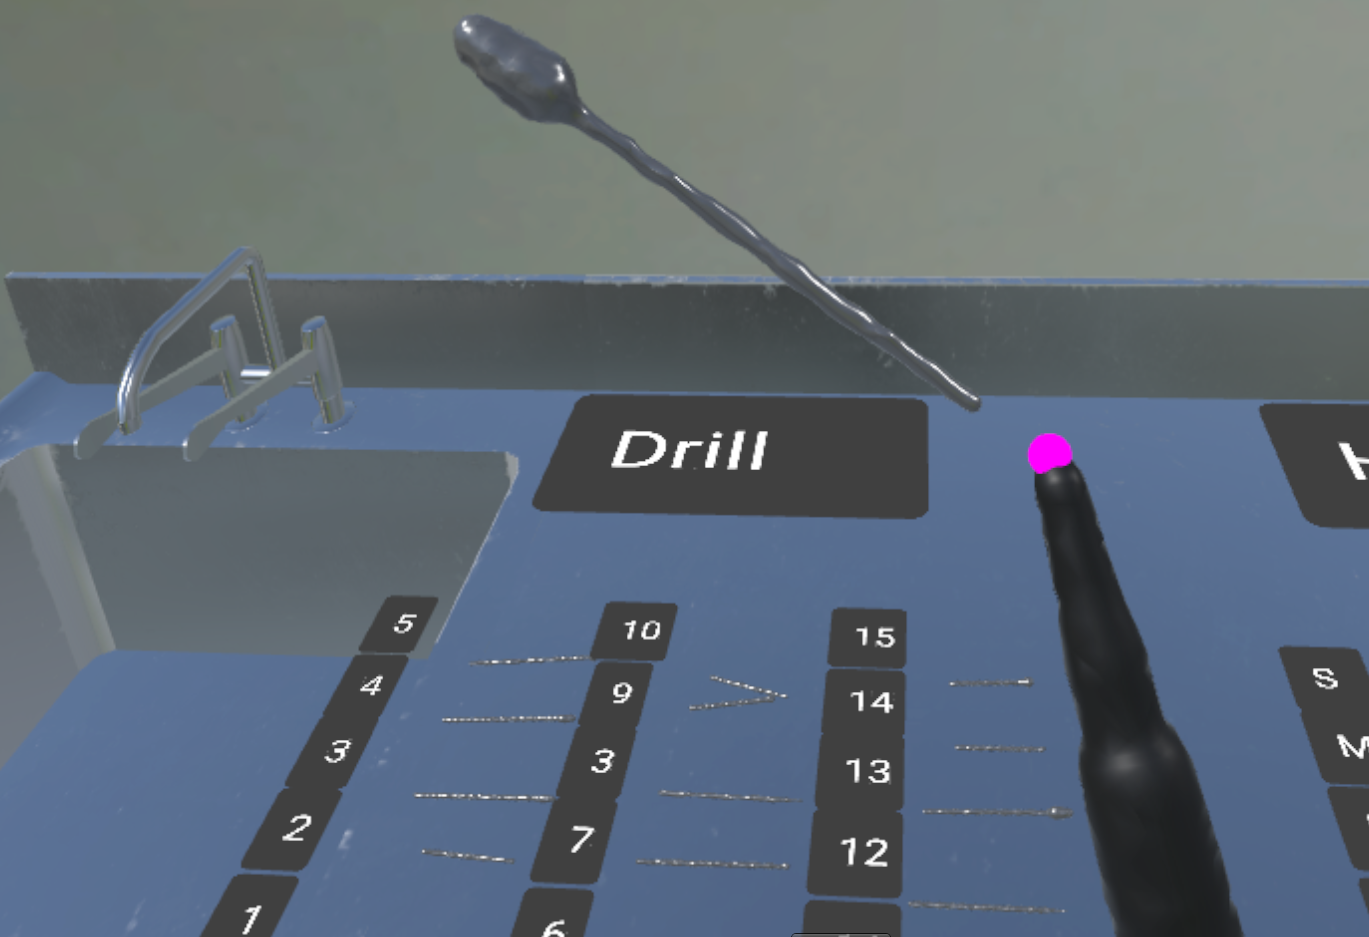
\includegraphics[width=200px]{images/implementation/features/procedures/drilling_attachment.png}
    \caption{\label{fig::FeatureDrillingAttachments}Process of attaching drill bit to the drill handle. With the right hand, the user performs the indicate action by touching 
    the respective button. With the other hand, the bit is picked up by grabbing it and moved into the pink sphere to attach the attachment.}
\end{figure}

In total, there are fifteen bits which can be used as an attachment for the drilling procedure.
Bits are modeled after their real counterparts in UHA.
They differ in size, length and width.
A visual signal is shown to the user while the indicate action is performed on the hand holding the drill handle.
By moving a drill bit to the visual indicator, the bit is attached to the handle (Figure \ref{fig::FeatureDrillingAttachments}).
Swapping out bits is performed by simply moving another bit into the indicator.
To perform the procedure, the drill handle must have a bit attached. 

\begin{figure}[ht]
    \centering
    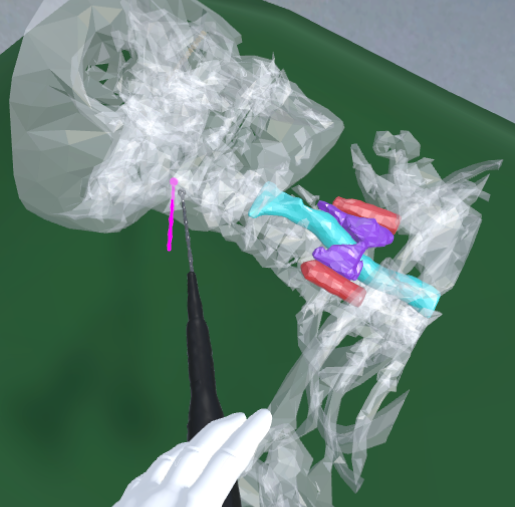
\includegraphics[width=200px]{images/implementation/features/procedures/drilling.png}
    \caption{\label{fig::FeatureDrilling}Drilling procedure. The pink object represents the last performed step, which was performed using the currently selected tool by pressing 
    the respective button all the way.}
\end{figure}

By triggering the perform action of the hand holding the drill, a copy of the currently attached drill bit is created and added to the project case. 
This copy has a different material, i.e. a pink material, to indicate that it is part of the project case (Figure \ref{fig::FeatureDrilling}).
Additionally, textual information about the currently attached drill bit will be stored in the project case, so that the exact procedure can be reproduced later (Requirements \ref{req::N3}, \ref{req::N5}).
The drill bit will not be removed on performing a procedure, so that multiple drilling steps can be performed consecutively.
When the drill is no longer needed, it can either be placed back on the instrument tray or the operating table for quick access.
Note that any instrument, excluding the osteosynthesis plates described later, can be placed anywhere in the OT.
\paragraph{Chiseling}

The \textbf{chiseling} procedure has two parts to it.
First, with one hand a chisel has to be chosen.
Users have a choice between a small, medium, large and extra large chisel to perform the procedure.
With the other hand, users then have to pick up the hammer.
Since this procedure requires users to hold two surgical instruments at the same time, this procedure can get cumbersome.
However, users can easily avoid this by placing the instruments on the operating table in the middle of the OT and repositioning afterwards (Figure \ref{fig::ChiselPrepare}).

\begin{figure}[ht]
    \centering
    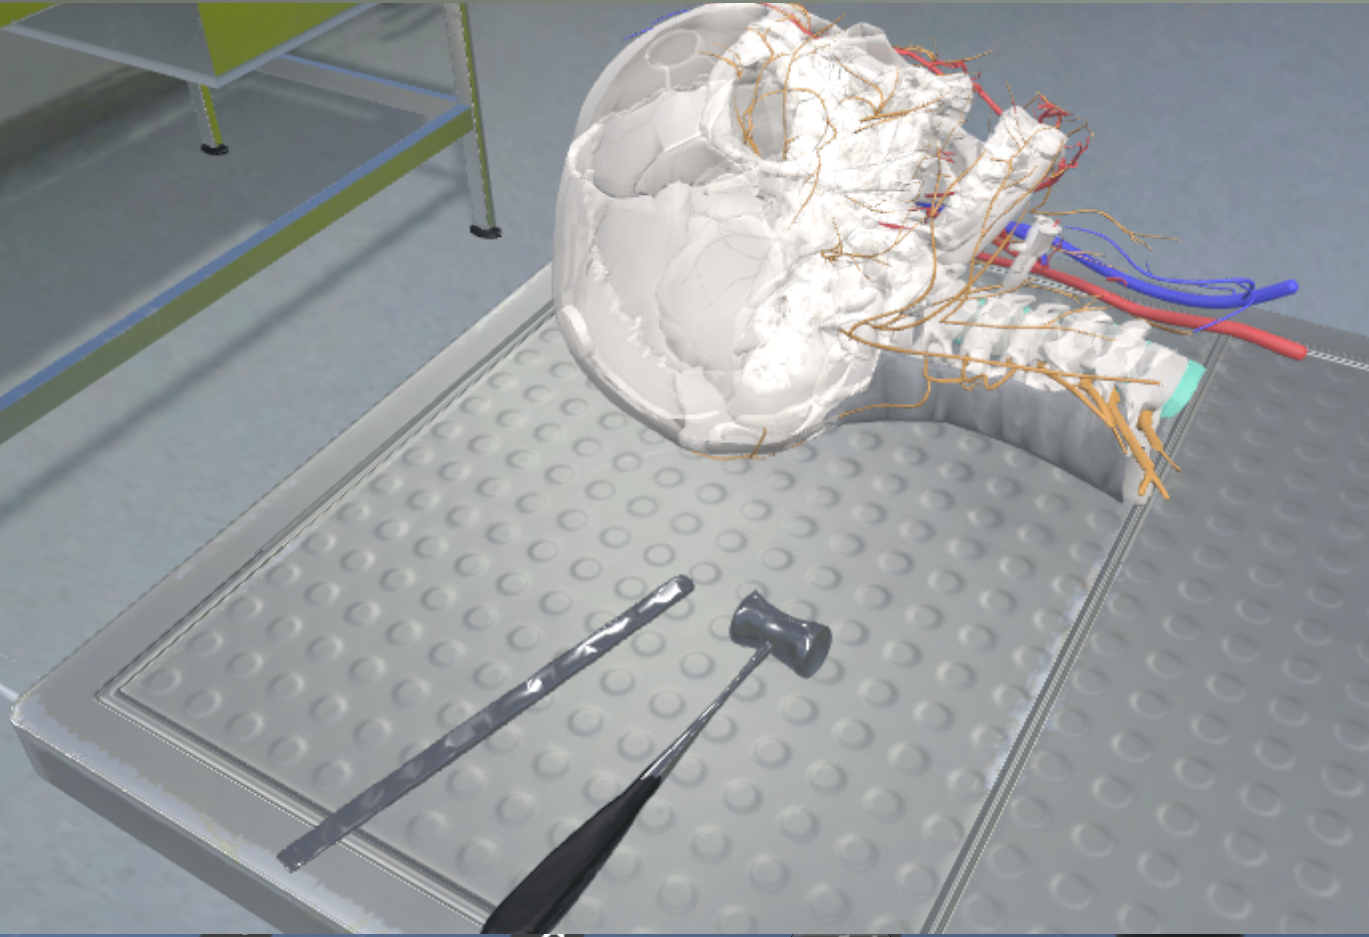
\includegraphics[width=\linewidth]{images/implementation/features/procedures/chisel_prepare.png}
    \caption{\label{fig::ChiselPrepare}The user prepares for the chiseling procedure by placing the instruments on the OT where the patient is located.
    indicators with the hammer in the other hand to perform the procedure.}
\end{figure}

When users have the perfect viewpoint, they can take up both instruments once again and start the procedure.
By pressing the indicate button on the hand where the chisel is located, rectangular indications at the top and bottom end of the chisel are shown to the user.
While these indications are active, the user has to perform a hammering motion with the hand holding the hammer.

\begin{figure}[ht]
    \centering
    \begin{minipage}{.5\textwidth}
      \centering
      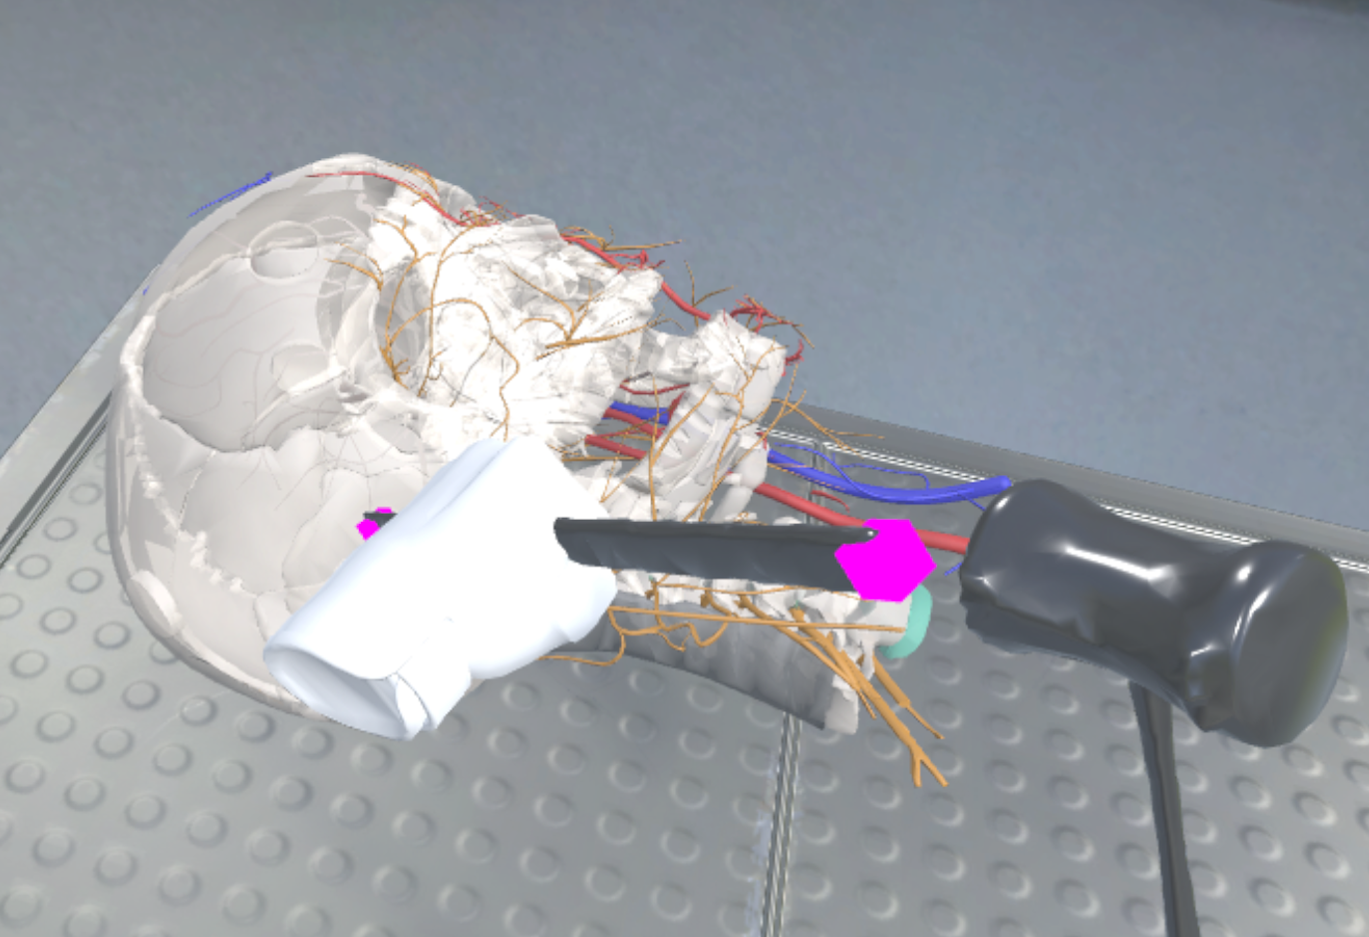
\includegraphics[width=0.99\linewidth]{images/implementation/features/procedures/chisel_1.png}
    \end{minipage}%
    \begin{minipage}{.5\textwidth}
      \centering
      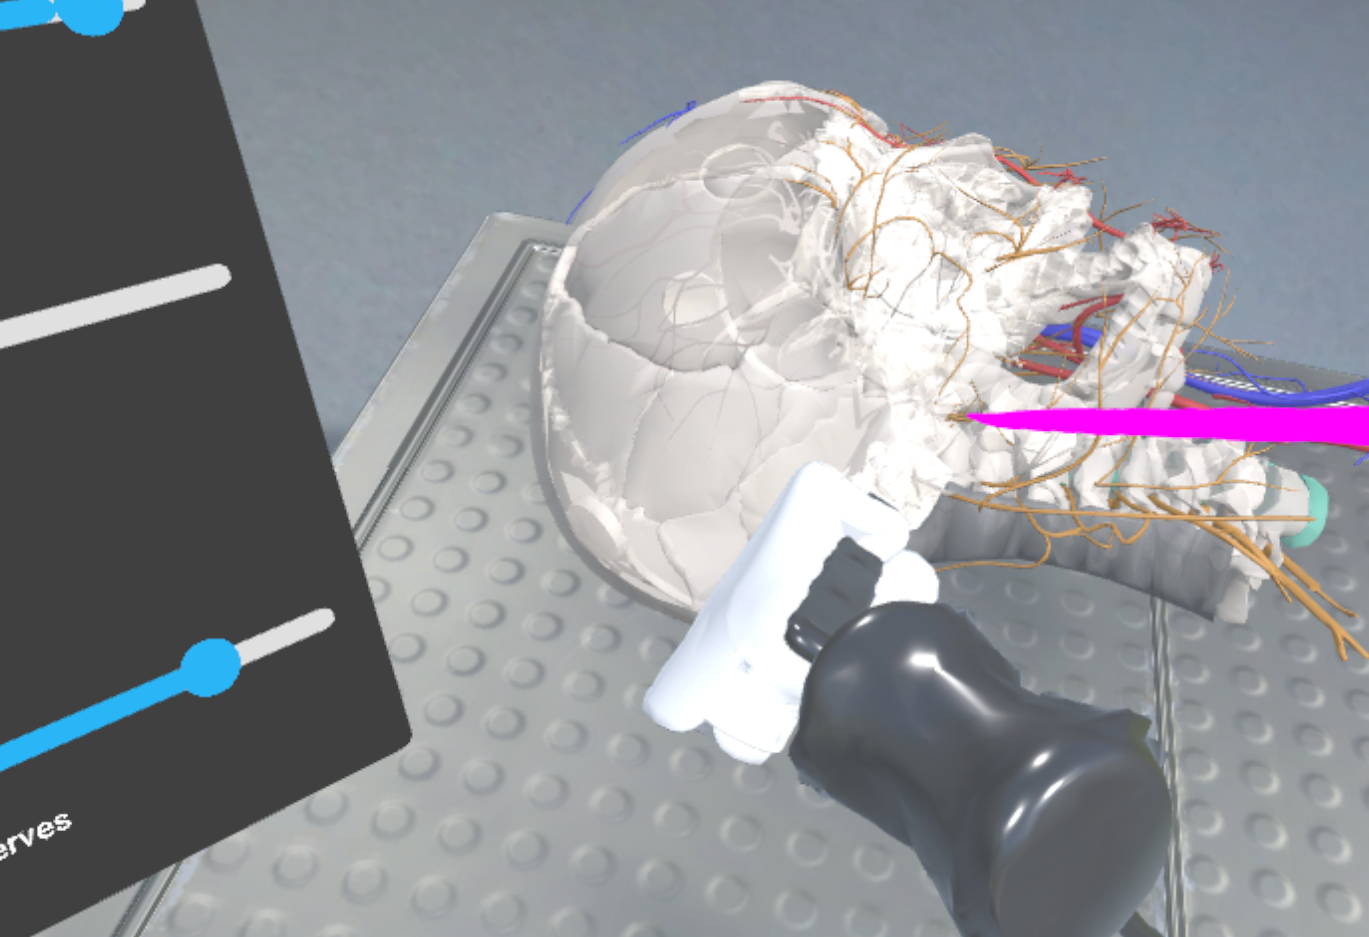
\includegraphics[width=0.99\linewidth]{images/implementation/features/procedures/chisel_2.png}
    \end{minipage}
    \caption{\label{fig::ChiselProcedure}Process of the chiseling procedure. Left: The users uses the indicate action with his left hand in preparation for the procedure. Right: After hammering on the indication on the chisel, the procedure has been performed and a step is generated.}
\end{figure}

When they hit the rectangular indicators located on the chisel, the chiseling procedure step is added to the project case in form of a modified copy of the hold chisel (Figure \ref{fig::ChiselProcedure}).
Here, information about the performed step is also included in the form of chisel size used for the procedure. 
\paragraph{Sawing}

\begin{figure}[ht]
    \centering
    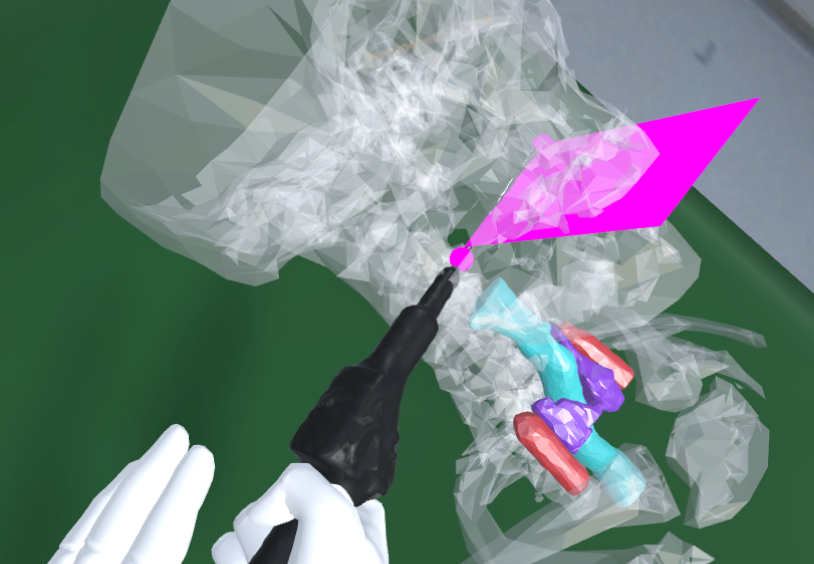
\includegraphics[width=200px]{images/implementation/features/procedures/bonesaw.png}
    \caption{\label{fig::FeatureBoneSaw}Bonesaw Procedure}
\end{figure}

The \textbf{sawing} procedure is performed by picking up the bonesaw.
Touch the controller will show two indications to the user (Figure \ref{fig::FeatureBoneSaw}).
The procedure is performed by first pressing down the trigger button and then letting go of it.
When letting go of the trigger button, a two dimensianal plane is created in the three dimensional space by using four points.
Two of these points are created when pressing down, and the other two when letting go of the trigger button.
A plane is then created with which the user can reproduce the way in which the bonesaw has been moved.
Arbitrary cutting shapes can be created by breaking them down into two-dimensional shapes and performing multiple movements.
\paragraph{Milling}

\begin{figure}[ht]
    \centering
    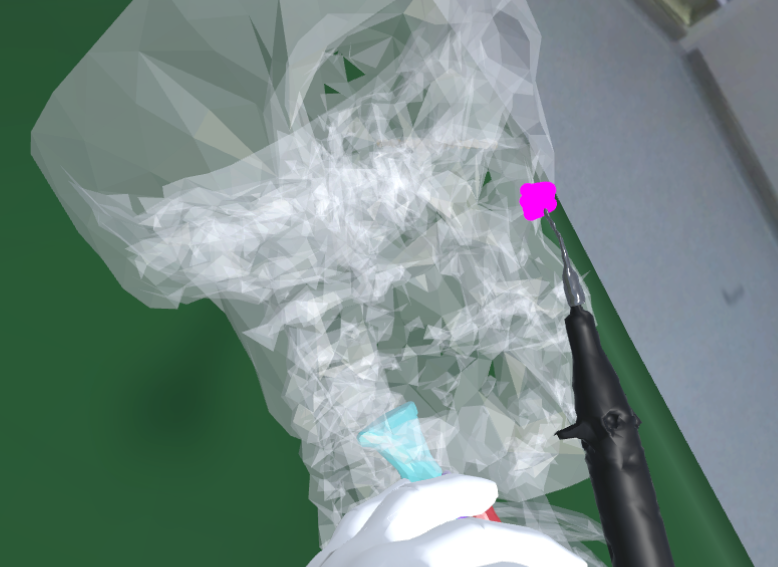
\includegraphics[width=200px]{images/implementation/features/procedures/piezo.png}
    \caption{\label{fig::FeaturePiezo}Milling procedure. Holding down the trigger button will draw little spheres until the button is released. The resulting object represents the volumetric space which is to be milled.}
\end{figure}

The \textbf{milling} operation is performed by grabbing the piezo instrument.
The indicator for the piezo is at the tip of the instrument, indicating which area will be milled.
While the "perform" button is being held down, little spheres are being drawn at the tip of the instrument \ref{fig::FeaturePiezo}.
When the button is released, the shapes are combined into a single 3D model and added as a project step.
The resulting object represents the volumetric space which has to be milled in the procedure.
The procedure can be reconstructed by "milling" the same 3D space in the virtual operating room.
\begin{figure}[ht!]
    \centering
    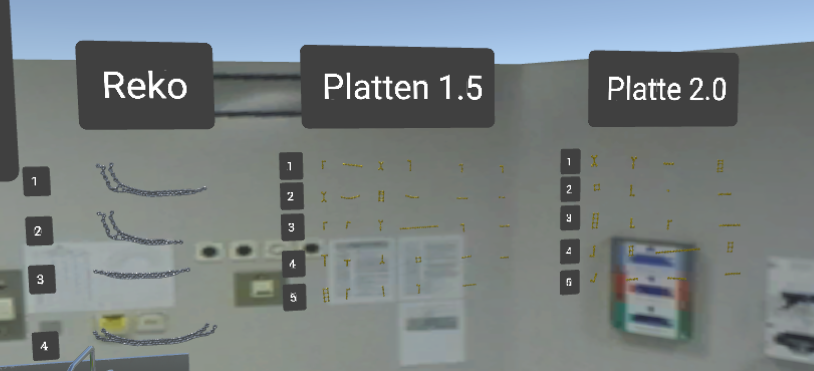
\includegraphics[width=\linewidth]{images/implementation/features/procedures/metal_plates_1.png}
    \caption{\label{fig::FeatureMetalPlate} Osteosynthesis Plates Overview}
\end{figure}

The osteosynthesis plates procedure consists of two steps before adding it as a step to the project case.
First, users have to chose which plate to use (Figure \ref{fig::FeatureMetalPlate}).
The user can chose from four reconstruction plates, 29 1.5mm plates and 20 2.0mm plates (Firma Angeben, osteosynthesis plates).
The optimal plates to use vary due to the pathology of the patient and the previously performed procedures.
After selecting the proper plate, a number of indicators will show to the user (Figure \ref{fig::FeatureMetalPlate2}).
In the context of the osteosynthesis plates, these indicators are "control points", with which the user can bend and twist the plates.
Bending and twisting is performed by chosing a control point via hovering them with the users free hand and grabbing them.
Then, the user has to translate and rotate the control point in the desired manner.
\begin{figure}
  \centering
  \begin{minipage}{.5\textwidth}
    \centering
    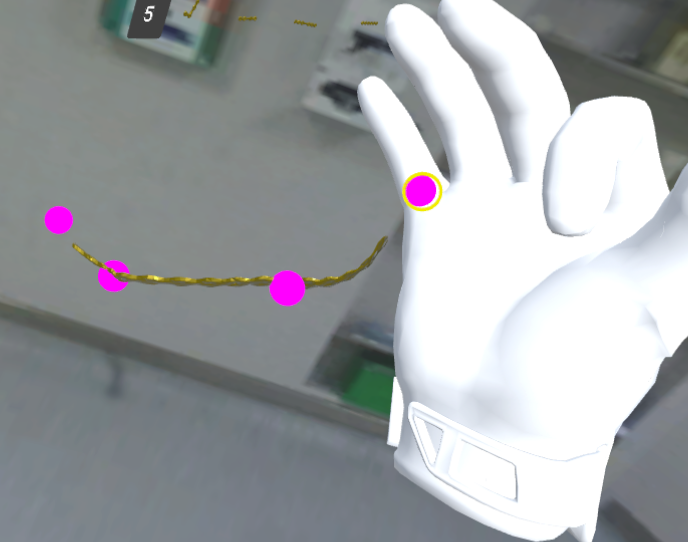
\includegraphics[width=0.95\linewidth]{images/implementation/features/procedures/metal_plates_2.png}
  \end{minipage}%
  \begin{minipage}{.5\textwidth}
    \centering
    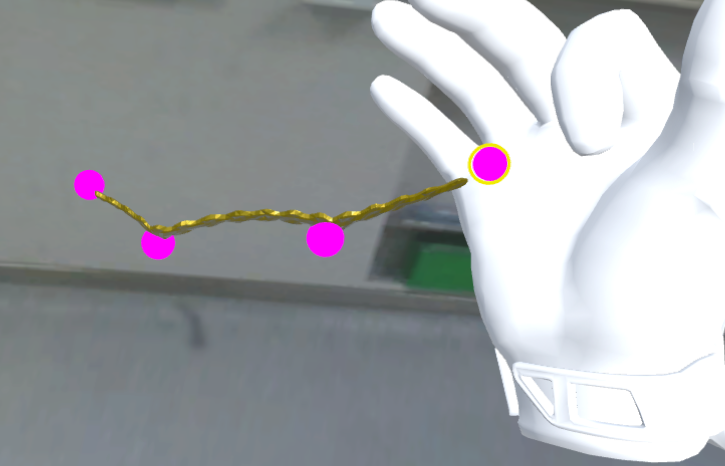
\includegraphics[width=0.95\linewidth]{images/implementation/features/procedures/metal_plates_3.png}
  \end{minipage}
  \caption{\label{fig::FeatureMetalPlate2}Osteosynthesis Plates Modifications. User can translate and rotate "control points" to perform modifications to the plates shape} 
\end{figure}

The user can then observe in which way this has affected the shape of the metal plate and either position the plate on the patient or perform more modifications to the plates via controlpoints.
The correct modification of the metal plates differs quite a lot from real life modifications to the plates.
However even though there is a slight learning curve to it, the modification is consistent and predictable (Figure \ref{fig::FeatureMetalPlate2}).


\begin{figure}[ht!]
    \centering
    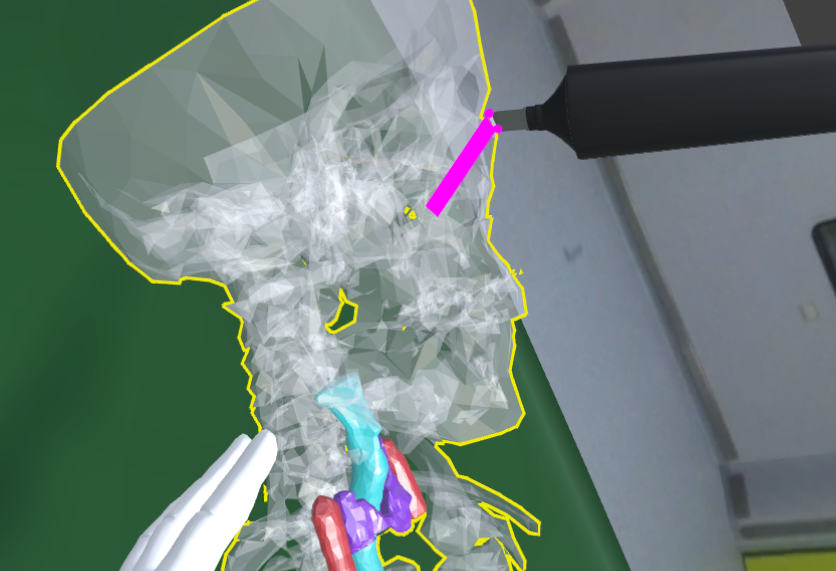
\includegraphics[width=\linewidth]{images/implementation/features/procedures/marker.png}
    \caption{\label{fig::FeatureMarker}Marker Procedure}
\end{figure}

The marking procedure is similar to the bonesaw procedure, meaning that rectangular shapes are drawed into the three dimensianal space (Figure \ref{fig::FeatureMarker}).
However, here the created shapes are much thinner.
In contrast to the bonesaw, the virtual hands of the user are also disabled here.
This way, the user can decide to hold the marker in the optimal way.
Since the main objective is marking specific spots on the patient, this is the natural approach.
\section{\label{sec::InteractionFlow}Interaction Flow}
At this point, the aforementioned six procedures are implemented in the system.
However, as described in Section \ref{sec::Architecture}, the system is extensible in the regard that new instruments can be implemented.
Currently, the implemented instruments are based on the workflow of OMF surgeons of the UHA: Users can perform drilling, hammer and chisel, bonesaw and milling operations.
Additionally, users can place markings and osteosynthesis plates on the virtual patient.
\\ To perform procedures, a project case has to be loaded first, as described in Section \ref{sec::GraphicalUserInterface}.
In the sense of SteamVRs interaction system described in Section \ref{sec::Architecture}, for each procedure there is an 'indicate' action when the user touches the 'perform' button, as well as an 'perform' action when the user presses the button all the way.
This way, users get a visual feedback when they are about to perform a procedure, as well as having visual indications of where the procedure will start (i.e. tip of the surgical instrument).
After described each procedure individually, how the procedures come together to create the steps for a procedure will be shortly desctribed.
\\ Each procedure will add a step to the project case.
In the sense of the VR-AR-based workflow described in Section \ref{sec::Workflow}, project cases can then be loaded into both parts of the workflow.
The steps are added to the hierarchy of the patient's 3D model and are identified as a step by name.
Through using this kind of approach, extensibility is guaranteed as each new instrument simply has to add some kind of geometry as a step to the project case (Requirements \ref{req::N8}, \ref{req::F3.7}).
It follows that any kind of procedure can then be imported into the AR workflow, even without touching the application.
\\ When a procedure is performed, users get voice feedback confirming that a step has been added to the project case.
Users can also navigate the project cases steps by using the VUIs commands, so that navigation through the steps of the procedure can be done while holding surgical instruments (Requirements \ref{req::N1}, \ref{req::F3.7}).
\\ For some of the surgical instruments, the user representation of the hand will be shown, for others not.
When a surgical instrument has this feature implemented, it is guaranteed that the instrument will always be grabbed and positioned in the same position on the hand, meaning the handgrip will always be the same.
However, in some cases, f.e. sawing with the bonesaw, this feature would prevent users from switching the handgrip of the surgical instrument. 
Therefore, for some instruments, this feature was removed.
Users will not see their virtual hands on the surgical instrument, but can chose to hold it however they want.
The virtual hands will be hidden while holding the instrument, however the instrument still represents the users hand position.
This way, the handgrip of the instrument can be adapted as users see fit.
The decision, on which was decided if hands should be hidden when grabbing an instrument, was made by a trial and error approach with the help of a physician's opinion on whether this features was useful.
The procedure specific implementation will be thoroughly described in the following.

\paragraph{Drilling}

The \textbf{drilling} operation is performed by first picking up the drill handle from the instrument tray via the grabbing action (Figure \ref{fig::FeatureDrillingAttachments}).
Since drills are typically held in a number of different ways, the handgrip of the drill handle is adjustable.
Therefore, the virtual hand will not be displayed while holding the drill.
The instrument tray is located next to the operating table, where the patient's model will initially be positioned.
The drill handle initially has no attachment; users have to attach a drill bit first.

\begin{figure}[ht]
    \centering
    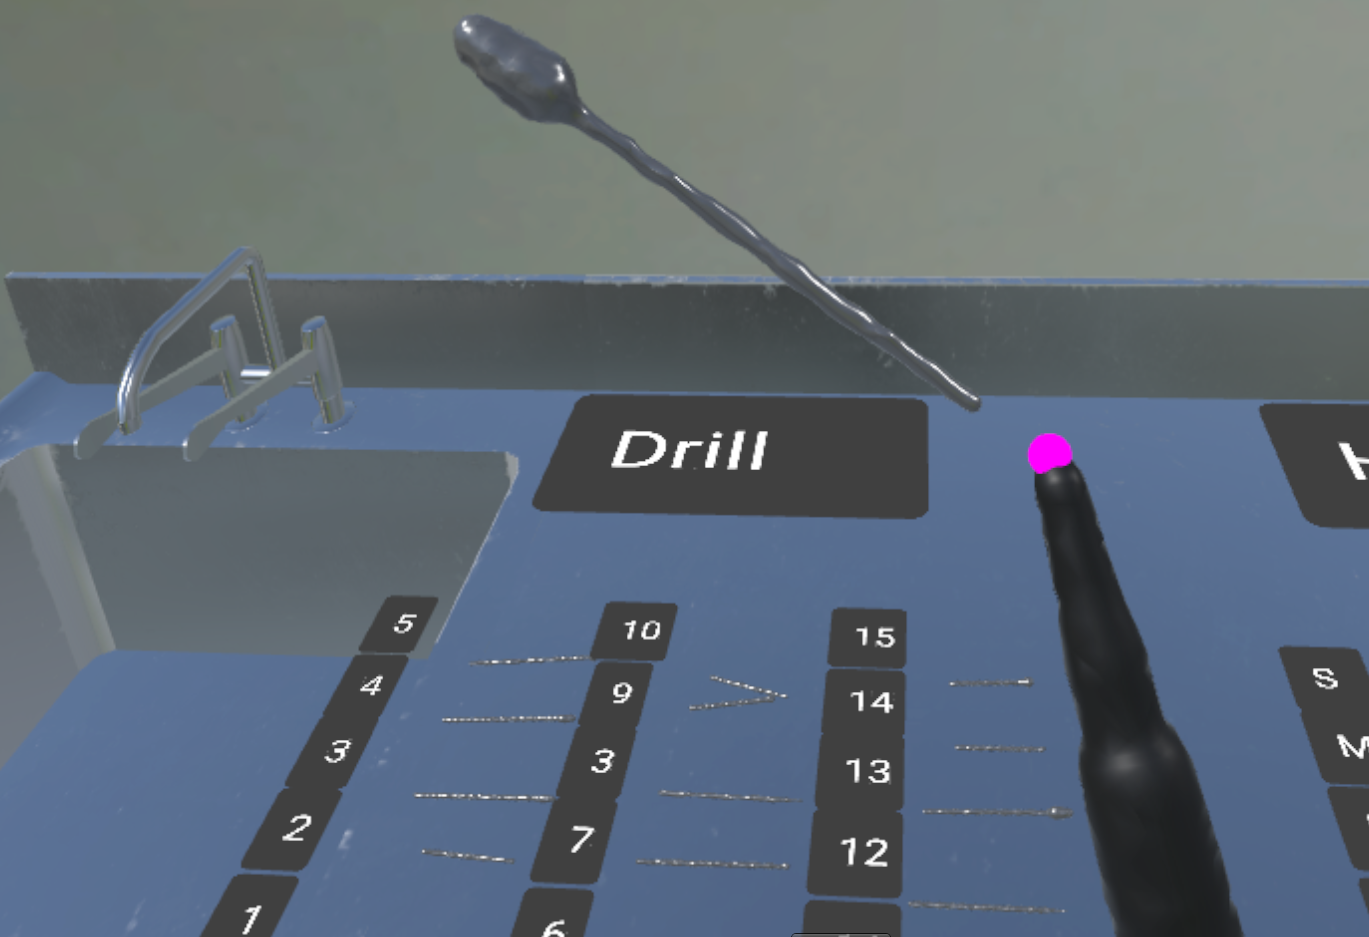
\includegraphics[width=200px]{images/implementation/features/procedures/drilling_attachment.png}
    \caption{\label{fig::FeatureDrillingAttachments}Process of attaching drill bit to the drill handle. With the right hand, the user performs the indicate action by touching 
    the respective button. With the other hand, the bit is picked up by grabbing it and moved into the pink sphere to attach the attachment.}
\end{figure}

In total, there are fifteen bits which can be used as an attachment for the drilling procedure.
Bits are modeled after their real counterparts in UHA.
They differ in size, length and width.
A visual signal is shown to the user while the indicate action is performed on the hand holding the drill handle.
By moving a drill bit to the visual indicator, the bit is attached to the handle (Figure \ref{fig::FeatureDrillingAttachments}).
Swapping out bits is performed by simply moving another bit into the indicator.
To perform the procedure, the drill handle must have a bit attached. 

\begin{figure}[ht]
    \centering
    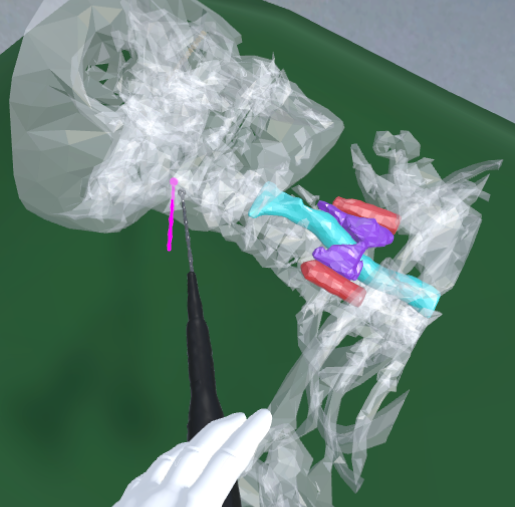
\includegraphics[width=200px]{images/implementation/features/procedures/drilling.png}
    \caption{\label{fig::FeatureDrilling}Drilling procedure. The pink object represents the last performed step, which was performed using the currently selected tool by pressing 
    the respective button all the way.}
\end{figure}

By triggering the perform action of the hand holding the drill, a copy of the currently attached drill bit is created and added to the project case. 
This copy has a different material, i.e. a pink material, to indicate that it is part of the project case (Figure \ref{fig::FeatureDrilling}).
Additionally, textual information about the currently attached drill bit will be stored in the project case, so that the exact procedure can be reproduced later (Requirements \ref{req::N3}, \ref{req::N5}).
The drill bit will not be removed on performing a procedure, so that multiple drilling steps can be performed consecutively.
When the drill is no longer needed, it can either be placed back on the instrument tray or the operating table for quick access.
Note that any instrument, excluding the osteosynthesis plates described later, can be placed anywhere in the OT.
\paragraph{Chiseling}

The \textbf{chiseling} procedure has two parts to it.
First, with one hand a chisel has to be chosen.
Users have a choice between a small, medium, large and extra large chisel to perform the procedure.
With the other hand, users then have to pick up the hammer.
Since this procedure requires users to hold two surgical instruments at the same time, this procedure can get cumbersome.
However, users can easily avoid this by placing the instruments on the operating table in the middle of the OT and repositioning afterwards (Figure \ref{fig::ChiselPrepare}).

\begin{figure}[ht]
    \centering
    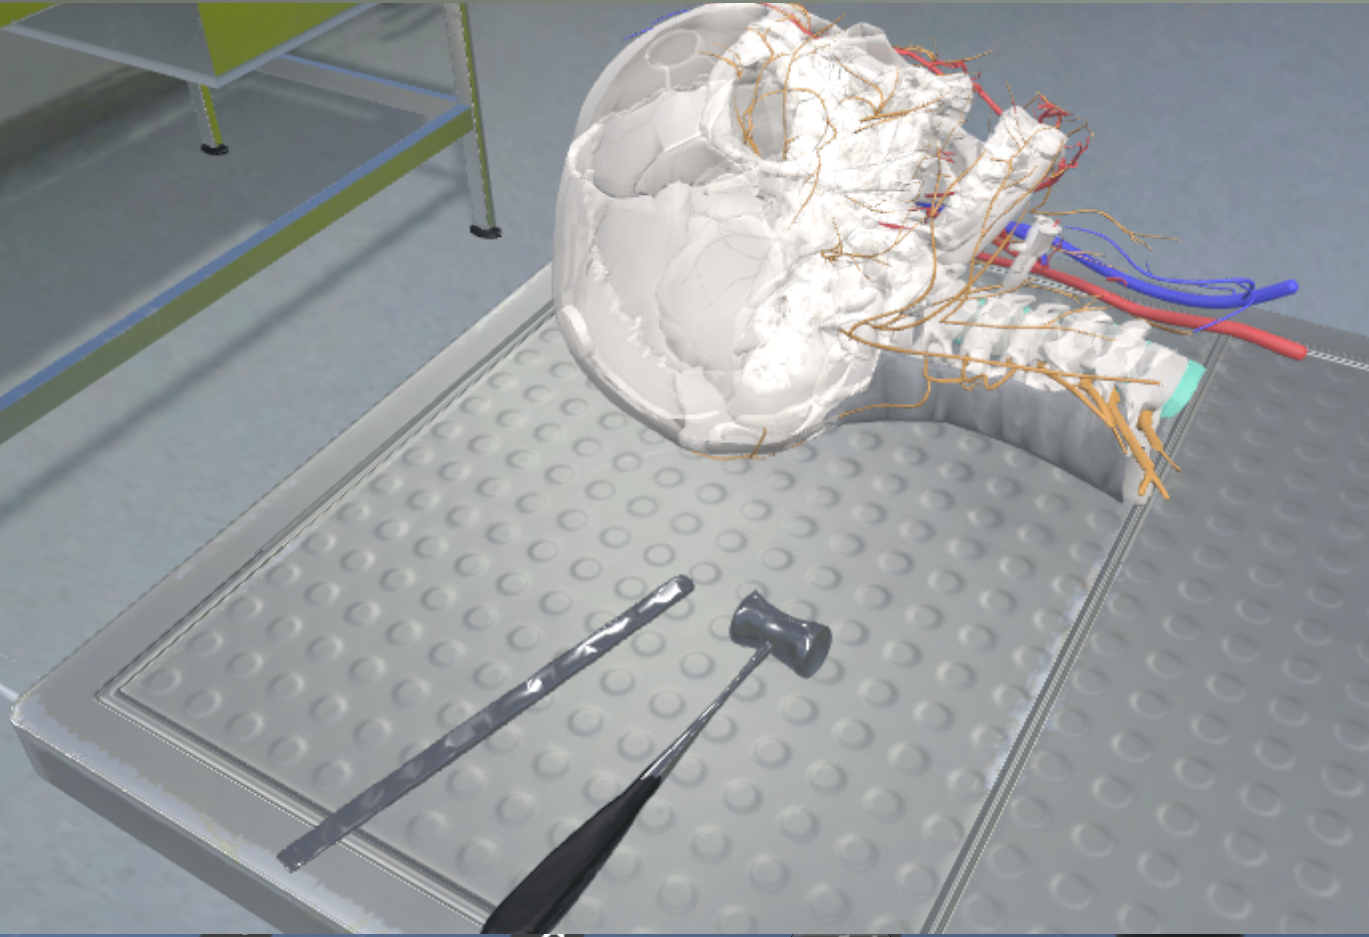
\includegraphics[width=\linewidth]{images/implementation/features/procedures/chisel_prepare.png}
    \caption{\label{fig::ChiselPrepare}The user prepares for the chiseling procedure by placing the instruments on the OT where the patient is located.
    indicators with the hammer in the other hand to perform the procedure.}
\end{figure}

When users have the perfect viewpoint, they can take up both instruments once again and start the procedure.
By pressing the indicate button on the hand where the chisel is located, rectangular indications at the top and bottom end of the chisel are shown to the user.
While these indications are active, the user has to perform a hammering motion with the hand holding the hammer.

\begin{figure}[ht]
    \centering
    \begin{minipage}{.5\textwidth}
      \centering
      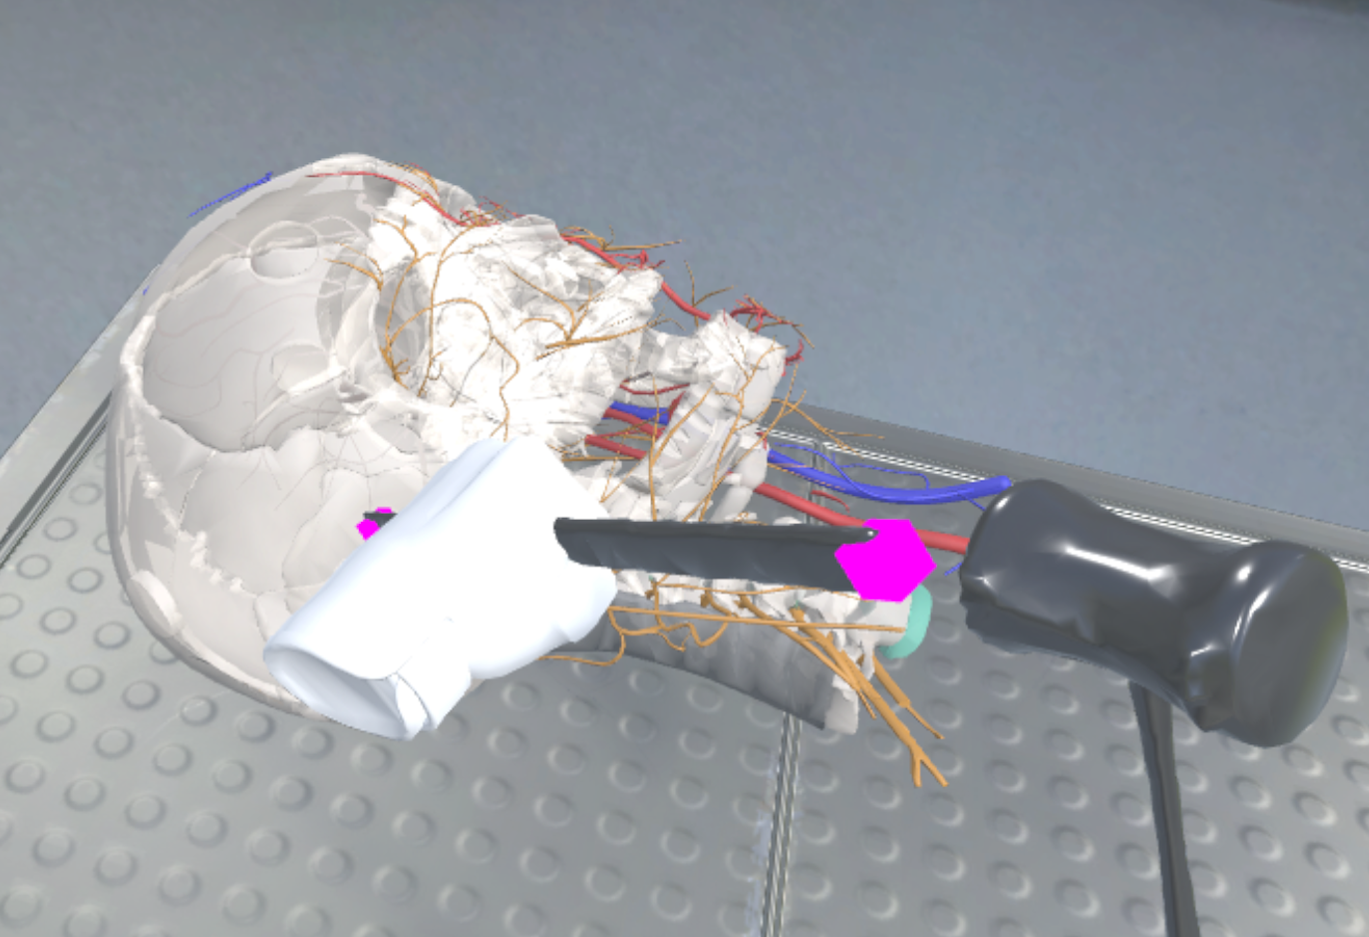
\includegraphics[width=0.99\linewidth]{images/implementation/features/procedures/chisel_1.png}
    \end{minipage}%
    \begin{minipage}{.5\textwidth}
      \centering
      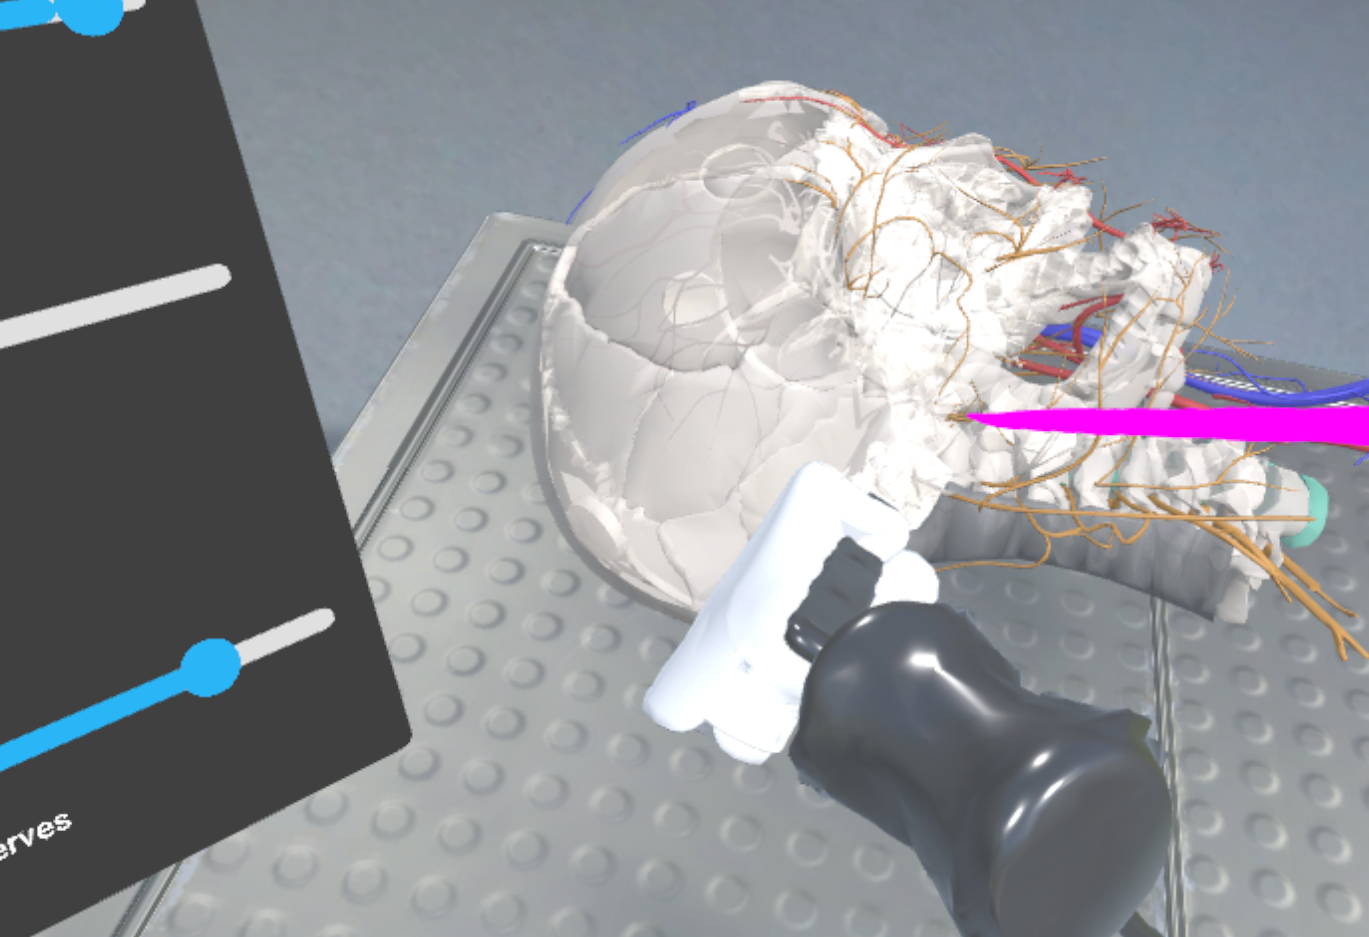
\includegraphics[width=0.99\linewidth]{images/implementation/features/procedures/chisel_2.png}
    \end{minipage}
    \caption{\label{fig::ChiselProcedure}Process of the chiseling procedure. Left: The users uses the indicate action with his left hand in preparation for the procedure. Right: After hammering on the indication on the chisel, the procedure has been performed and a step is generated.}
\end{figure}

When they hit the rectangular indicators located on the chisel, the chiseling procedure step is added to the project case in form of a modified copy of the hold chisel (Figure \ref{fig::ChiselProcedure}).
Here, information about the performed step is also included in the form of chisel size used for the procedure. 
\paragraph{Sawing}

\begin{figure}[ht]
    \centering
    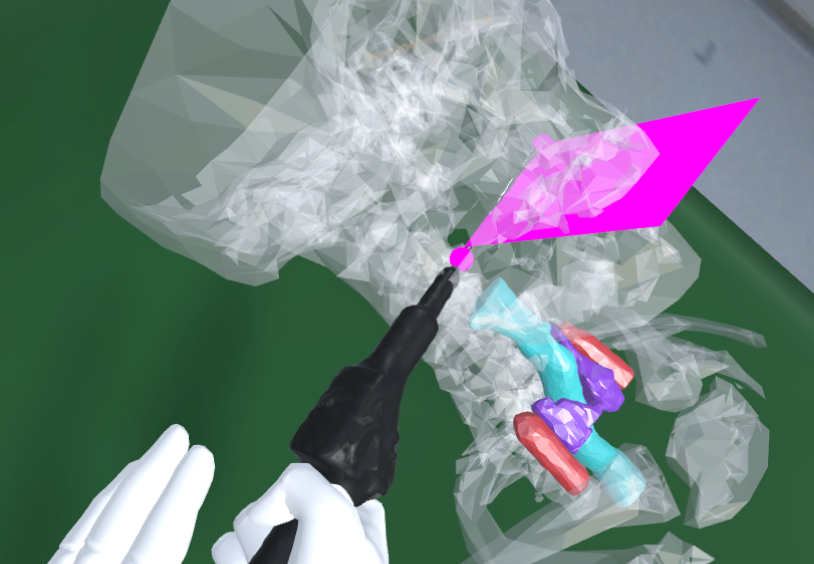
\includegraphics[width=200px]{images/implementation/features/procedures/bonesaw.png}
    \caption{\label{fig::FeatureBoneSaw}Bonesaw Procedure}
\end{figure}

The \textbf{sawing} procedure is performed by picking up the bonesaw.
Touch the controller will show two indications to the user (Figure \ref{fig::FeatureBoneSaw}).
The procedure is performed by first pressing down the trigger button and then letting go of it.
When letting go of the trigger button, a two dimensianal plane is created in the three dimensional space by using four points.
Two of these points are created when pressing down, and the other two when letting go of the trigger button.
A plane is then created with which the user can reproduce the way in which the bonesaw has been moved.
Arbitrary cutting shapes can be created by breaking them down into two-dimensional shapes and performing multiple movements.
\paragraph{Milling}

\begin{figure}[ht]
    \centering
    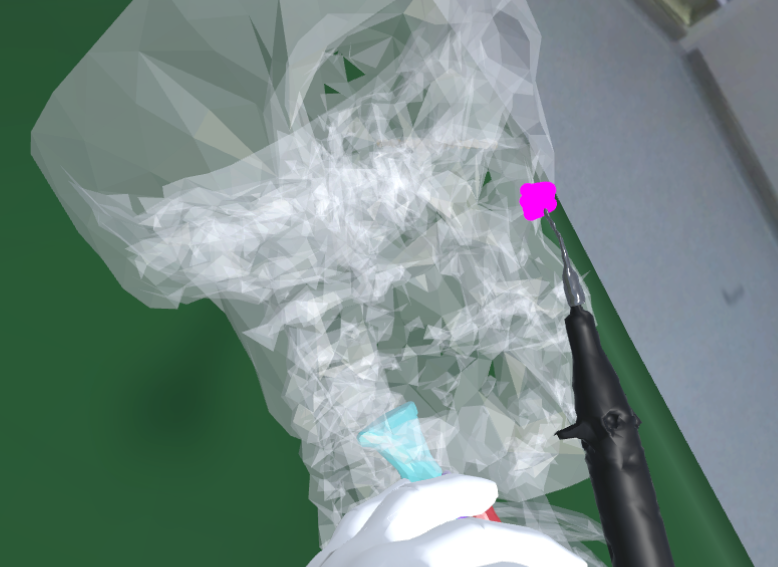
\includegraphics[width=200px]{images/implementation/features/procedures/piezo.png}
    \caption{\label{fig::FeaturePiezo}Milling procedure. Holding down the trigger button will draw little spheres until the button is released. The resulting object represents the volumetric space which is to be milled.}
\end{figure}

The \textbf{milling} operation is performed by grabbing the piezo instrument.
The indicator for the piezo is at the tip of the instrument, indicating which area will be milled.
While the "perform" button is being held down, little spheres are being drawn at the tip of the instrument \ref{fig::FeaturePiezo}.
When the button is released, the shapes are combined into a single 3D model and added as a project step.
The resulting object represents the volumetric space which has to be milled in the procedure.
The procedure can be reconstructed by "milling" the same 3D space in the virtual operating room.
\begin{figure}[ht!]
    \centering
    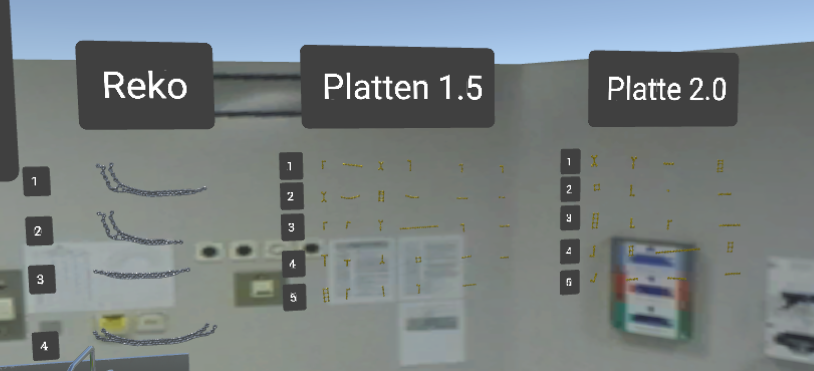
\includegraphics[width=\linewidth]{images/implementation/features/procedures/metal_plates_1.png}
    \caption{\label{fig::FeatureMetalPlate} Osteosynthesis Plates Overview}
\end{figure}

The osteosynthesis plates procedure consists of two steps before adding it as a step to the project case.
First, users have to chose which plate to use (Figure \ref{fig::FeatureMetalPlate}).
The user can chose from four reconstruction plates, 29 1.5mm plates and 20 2.0mm plates (Firma Angeben, osteosynthesis plates).
The optimal plates to use vary due to the pathology of the patient and the previously performed procedures.
After selecting the proper plate, a number of indicators will show to the user (Figure \ref{fig::FeatureMetalPlate2}).
In the context of the osteosynthesis plates, these indicators are "control points", with which the user can bend and twist the plates.
Bending and twisting is performed by chosing a control point via hovering them with the users free hand and grabbing them.
Then, the user has to translate and rotate the control point in the desired manner.
\begin{figure}
  \centering
  \begin{minipage}{.5\textwidth}
    \centering
    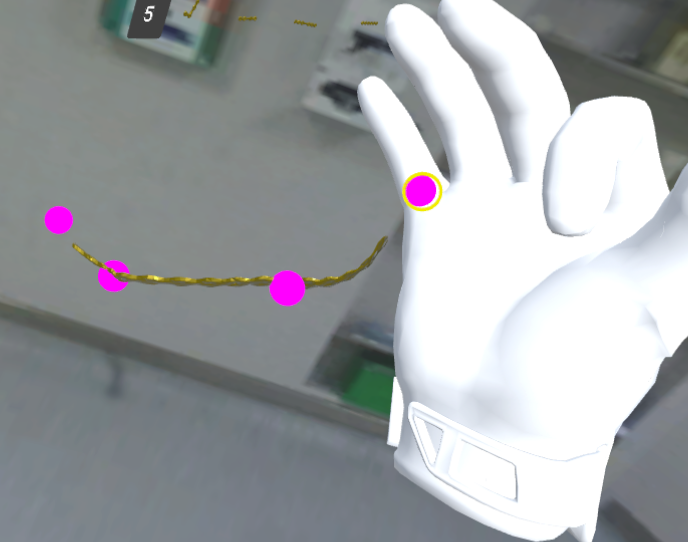
\includegraphics[width=0.95\linewidth]{images/implementation/features/procedures/metal_plates_2.png}
  \end{minipage}%
  \begin{minipage}{.5\textwidth}
    \centering
    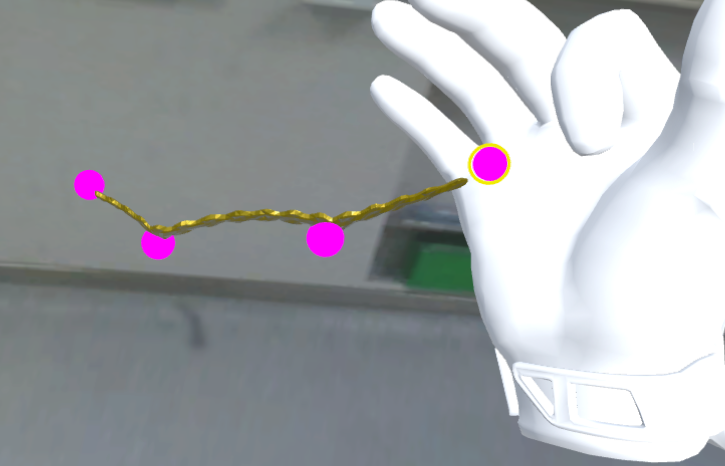
\includegraphics[width=0.95\linewidth]{images/implementation/features/procedures/metal_plates_3.png}
  \end{minipage}
  \caption{\label{fig::FeatureMetalPlate2}Osteosynthesis Plates Modifications. User can translate and rotate "control points" to perform modifications to the plates shape} 
\end{figure}

The user can then observe in which way this has affected the shape of the metal plate and either position the plate on the patient or perform more modifications to the plates via controlpoints.
The correct modification of the metal plates differs quite a lot from real life modifications to the plates.
However even though there is a slight learning curve to it, the modification is consistent and predictable (Figure \ref{fig::FeatureMetalPlate2}).


\begin{figure}[ht!]
    \centering
    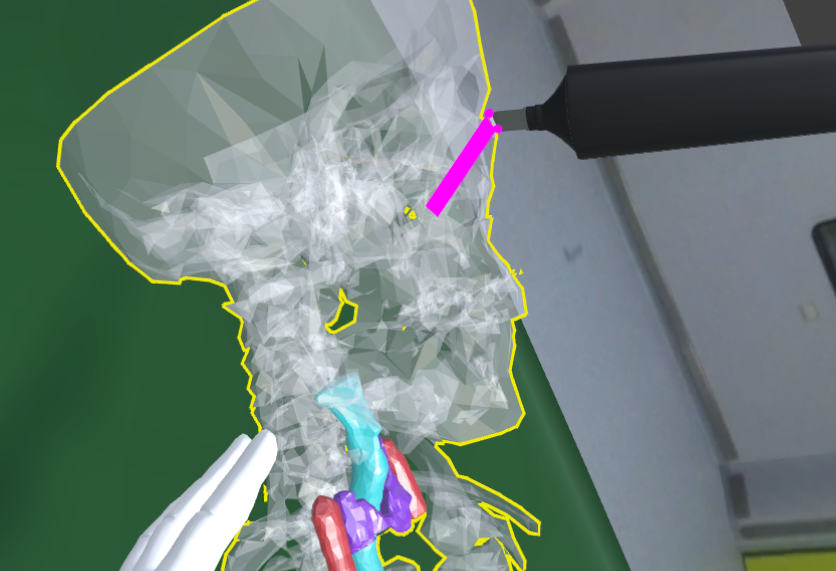
\includegraphics[width=\linewidth]{images/implementation/features/procedures/marker.png}
    \caption{\label{fig::FeatureMarker}Marker Procedure}
\end{figure}

The marking procedure is similar to the bonesaw procedure, meaning that rectangular shapes are drawed into the three dimensianal space (Figure \ref{fig::FeatureMarker}).
However, here the created shapes are much thinner.
In contrast to the bonesaw, the virtual hands of the user are also disabled here.
This way, the user can decide to hold the marker in the optimal way.
Since the main objective is marking specific spots on the patient, this is the natural approach.